% ==============================================================
% Relatório Final de Iniciação Científica — UFES / PIIC
% Subprojeto: Otimização Dinâmica de Rotas para Coleta de Resíduos
%             Sólidos: Adaptação do Algoritmo de Solomon com IoT
% Estudante: Emilly Lopes Das Neves   Orientadora: Maria Claudia Silva Boeres
%
% Relatório completo: formulação, invariantes de viabilidade, pseudocódigos,
% critérios de aceitação, calibração, estatística, resultados (sob o critério de
% parada por iterações sem melhoria) e aplicação no Digital Twin.
% Compilar com pdflatex (precisa dos pacotes algorithm e algorithmic); figuras em ../../results.
% ==============================================================
\documentclass[12pt, a4paper]{article}

\usepackage{graphicx,color}
\usepackage[dvipsnames]{xcolor,colortbl}
\usepackage[hidelinks]{hyperref}
\usepackage{anysize}
\usepackage{iftex}
\ifPDFTeX
  \usepackage[utf8]{inputenc}
  \usepackage[T1]{fontenc}
\else
  \usepackage{fontspec}
\fi
\usepackage{fancyhdr}
\usepackage{array}
\usepackage{amsmath,amssymb}
\usepackage{titlesec}
\ifPDFTeX
  \usepackage{mathptmx}
\fi
\usepackage{booktabs}
\usepackage{float}
\usepackage{longtable}
\usepackage{multirow}
\usepackage{algorithm}
\usepackage{algorithmic}
\usepackage{enumitem}
\usepackage{caption}
\usepackage{subcaption}

% Pseudocódigo em português (pacote algorithmic; mesmo estilo do modelo ex_pseudo_codigo.tex).
\floatname{algorithm}{Algoritmo}
\renewcommand{\algorithmicrequire}{\textbf{Entrada:}}
\renewcommand{\algorithmicensure}{\textbf{Saída:}}
\renewcommand{\algorithmicwhile}{\textbf{enquanto}}
\renewcommand{\algorithmicdo}{\textbf{faça}}
\renewcommand{\algorithmicend}{\textbf{fim}}
\renewcommand{\algorithmicif}{\textbf{se}}
\renewcommand{\algorithmicthen}{\textbf{então}}
\renewcommand{\algorithmicelse}{\textbf{senão}}
\renewcommand{\algorithmicelsif}{\textbf{senão se}}
\renewcommand{\algorithmicfor}{\textbf{para}}
\renewcommand{\algorithmicforall}{\textbf{para todo}}
\renewcommand{\algorithmicreturn}{\textbf{retorne}}
\renewcommand{\algorithmicrepeat}{\textbf{repita}}
\renewcommand{\algorithmicuntil}{\textbf{até}}
\renewcommand{\algorithmiccomment}[1]{\hfill\(\triangleright\)~\textit{#1}}

\ifPDFTeX
  \usepackage{helvet}
  \renewcommand{\familydefault}{\sfdefault}
\else
  % Arial quando existir (Windows/macOS); Liberation Sans e a equivalente
  % metrica aberta, presente nas distribuicoes Linux.
  \IfFontExistsTF{Arial}
    {\setmainfont{Arial}\setsansfont{Arial}}
    {\setmainfont{Liberation Sans}\setsansfont{Liberation Sans}}
  \renewcommand{\familydefault}{\sfdefault}
\fi
\usepackage{setspace}\onehalfspacing
\usepackage{parskip}\setlength{\parindent}{0pt}\setlength{\parskip}{6pt}
\usepackage{natbib}

\titleformat{\section}{\normalfont\fontsize{14}{16}\bfseries}{\thesection}{1em}{}[{\titlerule[0.8pt]}]
\captionsetup{font={footnotesize}, labelsep=endash, singlelinecheck=false, justification=raggedright}

\usepackage{tabularx}
\newcolumntype{L}[1]{>{\raggedright\arraybackslash}p{#1}}

\usepackage[a4paper, left=30mm, top=30mm, right=20mm, bottom=20mm, includehead, headsep=25mm, headheight=35pt]{geometry}
\addtolength{\voffset}{-25mm}\addtolength{\textheight}{25mm}
\pagestyle{fancy}\fancyhf{}
\fancyhead[R]{\fontsize{10}{12}\selectfont\color{Gray} Universidade Federal do Espírito Santo\\ Programa Institucional de Iniciação Científica\\ Relatório Final de Pesquisa\\ Ciência da Computação}
\renewcommand{\headrulewidth}{0pt}
\fancyfoot[R]{\thepage}\renewcommand{\footrulewidth}{0pt}

% Orçamento de parada declarado, uniforme (preenchido a partir de config/fixed_K.json).
\newcommand{\Kgrasp}{800}
\newcommand{\Krgrasp}{800}
\newcommand{\Ktabu}{800}


\begin{document}

% ---------------- Cabeçalho institucional ----------------
\bgroup\def\arraystretch{1.1}
\begin{tabularx}{\textwidth}{|>{\columncolor{gray!25}}L{59mm}|L{88mm}|}
\hline
{\bf Edital:} & {\bf Edital PIIC 2025/2026} \\ \hline
{\bf Área (CNPq):} & {\bf Ciência da Computação} \\ \hline
{\bf Subárea (CNPq):} & {\bf Metodologia e Técnicas da Computação} \\ \hline
{\bf Título do Projeto:} & {\bf Pesquisa Operacional e Inovação em Logística Regional} \\ \hline
{\bf Título do Subprojeto:} & {\bf Otimização Dinâmica de Rotas para Coleta de Resíduos Sólidos: Adaptação do Algoritmo de Solomon com Integração IoT} \\ \hline
{\bf Orientadora:} & {\bf Maria Claudia Silva Boeres} \\ \hline
{\bf Estudante:} & {\bf Emilly Lopes Das Neves} \\ \hline
\end{tabularx}\egroup
\vspace{4mm}

\begin{center}\textbf{\large Comparação experimental de cinco heurísticas clássicas para o VRPTW,\\ com aplicação à coleta de resíduos sólidos via Digital Twin}\end{center}
\vspace{2mm}

% ---------------- Resumo ----------------
\noindent\textbf{Resumo.} Este trabalho apresenta uma comparação experimental, sob condições controladas e reprodutíveis, de cinco heurísticas e meta-heurísticas clássicas para o Problema de Roteamento de Veículos com Janelas de Tempo (VRPTW): a heurística de inserção I1 de \citet{solomon1987algorithms}, a Descida em Vizinhança Variável (VND) \citep{hansen2001variable}, o GRASP \citep{feo1995greedy} nas formas fixa e reativa \citep{prais2000reactive}, e a Busca Tabu \citep{glover1989tabu}. Todos os métodos compartilham o mesmo núcleo (leitor de instâncias, função de distância, avaliador de viabilidade, conjunto de vizinhanças e gerador pseudoaleatório), de modo que as diferenças observadas decorram exclusivamente da estratégia de busca. A função-objetivo otimizada é a distância total sob a convenção do 12\textsuperscript{o} Desafio DIMACS; a contagem de veículos é reportada como medida secundária. Avaliamos as 56 instâncias de 100 clientes de Solomon, com calibração de parâmetros por \textit{irace} \citep{lopez2016irace} sob divisão treino/teste, parada por número de iterações sem melhoria, e comparação estatística por Friedman seguida do pós-teste de Nemenyi \citep{demsar2006statistical}. A viabilidade (cobertura de todos os clientes, capacidade e janelas de tempo) é garantida por construção e \emph{reverificada de forma independente} em todas as soluções. Por fim, um \textit{Digital Twin} aplica os algoritmos calibrados a um cenário de coleta de resíduos com localizações reais de Vitória/ES, como prova de conceito.

\medskip
\noindent\textbf{Palavras-chave:} VRPTW; meta-heurísticas; GRASP; Busca Tabu; comparação experimental; coleta de resíduos.

% ============================================================
\section{Introdução}\label{sec:intro}

A gestão de resíduos sólidos urbanos impõe desafios operacionais, econômicos e ambientais aos municípios. Sistemas convencionais de coleta, baseados em rotas fixas e frequências predeterminadas, geram deslocamentos desnecessários e respondem mal a situações de enchimento crítico dos recipientes \citep{pardini2020smart,lozano2018smart}. A literatura aponta que integrar monitoramento em tempo real e otimização de rotas pode tornar a coleta mais eficiente \citep{lozano2018smart,barth2023data}.

Este subprojeto de Iniciação Científica combina sensoriamento IoT via LoRaWAN \citep{ramson2021lorawan,de2021plataforma} com heurísticas baseadas no algoritmo de \citet{solomon1987algorithms} para o VRPTW, além de um \textit{Digital Twin} para simulação e visualização. A pergunta de pesquisa é: \emph{de que modo a comparação criteriosa de heurísticas clássicas para o VRPTW pode fundamentar um planejamento de coleta mais responsivo e eficiente, preservando a factibilidade temporal das rotas?}

A contribuição deste relatório é metodológica e experimental, organizada em três camadas: (i) um \textbf{\textit{benchmark} estático} sobre as instâncias clássicas de Solomon, que estabelece a base de comparação justa e calibra os algoritmos; (ii) uma \textbf{análise estatística} do desempenho relativo dos cinco métodos; e (iii) uma \textbf{aplicação dinâmica} (Digital Twin) que transfere os algoritmos calibrados a um cenário de coleta de resíduos. O \textit{benchmark} estático é a base metodológica sobre a qual a aplicação dinâmica se apoia: os mesmos operadores e parâmetros validados nas instâncias de Solomon são reaproveitados no Digital Twin.

% ============================================================
\section{O Problema de Roteamento com Janelas de Tempo}\label{sec:problema}

\subsection{Formulação}
Seja um grafo completo $G=(V,A)$, com $V=\{0,1,\dots,n\}$, em que o vértice $0$ é o depósito e $C=\{1,\dots,n\}$ são os clientes. A cada cliente $i$ associam-se: demanda $q_i\ge 0$, janela de tempo $[e_i,\ell_i]$ e tempo de serviço $s_i$. O depósito tem janela $[e_0,\ell_0]$ (o horizonte) e $q_0=s_0=0$. Uma frota homogênea de veículos de capacidade $Q$ parte e retorna ao depósito. A cada arco $(i,j)$ associam-se uma distância $d_{ij}$ e um tempo de viagem $t_{ij}$.

Uma \emph{rota} é uma sequência $r=\langle 0, c_1, \dots, c_m, 0\rangle$. Definindo o instante de chegada $a_{c_1}=t_{0,c_1}$ e, para $k>1$, o início de serviço $b_{c_{k}}=\max(a_{c_k},e_{c_k})$ com $a_{c_{k}}=b_{c_{k-1}}+s_{c_{k-1}}+t_{c_{k-1},c_k}$, a rota é \emph{viável} se
\begin{equation}
b_{c_k}\le \ell_{c_k}\ \ \forall k,\qquad
\sum_{k} q_{c_k}\le Q,\qquad
b_{c_m}+s_{c_m}+t_{c_m,0}\le \ell_0 .
\label{eq:viab}
\end{equation}
Uma \emph{solução} $S$ é um conjunto de rotas $\mathcal{R}(S)$ em que cada cliente é visitado \textbf{exatamente uma vez}. Suas duas grandezas de interesse são a \textbf{distância total} e o \textbf{número de veículos}:
\begin{equation}
D(S)=\sum_{r\in\mathcal{R}(S)}\ \sum_{(i,j)\in r} d_{ij},
\qquad
K(S)=|\mathcal{R}(S)|.
\label{eq:defs}
\end{equation}
O objetivo primário deste trabalho é minimizar a distância total $D(S)$, conforme detalhado na Seção~\ref{sec:objetivo}.

\subsection{Convenção de distância e função-objetivo}\label{sec:objetivo}
Adotamos a convenção do 12\textsuperscript{o} Desafio DIMACS para o VRPTW \citep{dimacs12vrptw}: a distância de cada arco é a euclidiana \textbf{truncada} a uma casa decimal, $d_{ij}=\lfloor 10\,e_{ij}\rfloor/10$ (com $e_{ij}$ a distância euclidiana), e o tempo de viagem é igual à distância ($t_{ij}=d_{ij}$). O truncamento é a padronização adotada pelo desafio para tornar custos comparáveis entre implementações; os resultados originais de \citet{solomon1987algorithms} foram computados em precisão total --- distinção relevante ao confrontar valores publicados sob convenções diferentes, discutida na Seção~\ref{sec:baseline}. As regras do desafio adotam explicitamente a minimização \emph{apenas da distância total} (não a hierarquia veículos$\rightarrow$distância): verifica-se que a solução respeita o número máximo de veículos disponíveis, mas não há bônus por usar menos. Essa convenção foi escolhida por ser o padrão internacional moderno do desafio e por ser \emph{verificável}: ela reproduz exatamente os custos das soluções de referência (Seção~\ref{sec:verificacao}). Formalmente, o objetivo otimizado pela busca é
\begin{equation}
\min_{S\ \text{viável}}\ D(S),
\label{eq:obj-dist}
\end{equation}
com a distância relatada a uma casa decimal e o número de veículos $K(S)$ como medida secundária. Essa formulação difere da hierarquia \emph{lexicográfica} clássica de \citet{solomon1987algorithms},
\begin{equation}
\operatorname*{lex\,min}_{S\ \text{viável}}\ \big(K(S),\ D(S)\big),
\label{eq:obj-lex}
\end{equation}
que minimiza \emph{primeiro} o número de veículos e, entre soluções de mesma frota, a distância. Sob a Equação~\eqref{eq:obj-dist}, a busca não minimiza o número de veículos diretamente; este é uma consequência da construção e só diminui quando um movimento entre rotas esvazia completamente uma rota. A Seção~\ref{sec:baseline} discute, de forma transparente, as implicações dessa escolha sobre a comparação com os melhores valores conhecidos.

\subsection{Invariantes de viabilidade}\label{sec:invariantes}
Um requisito central deste trabalho é que \textbf{toda} solução produzida — pela construção \emph{e} por todo algoritmo de melhoria — satisfaça a Equação~\eqref{eq:viab} e a cobertura de clientes. Garantimos isso por três mecanismos redundantes:
\begin{enumerate}[noitemsep]
\item \textbf{Avaliação por rota.} Cada rota mantém os vetores de chegada, início e partida, recalculados a cada modificação; a viabilidade da janela e da capacidade é verificada nessa passagem.
\item \textbf{Critério Push Forward.} Para inserções, calcula-se o \emph{folga} (\textit{slack}) máximo de deslocamento para frente de cada cliente sem violar a própria janela nem as subsequentes; uma inserção só é aceita se o atraso que provoca couber nessa folga. Isso permite testar viabilidade em $O(1)$ por posição candidata \citep{solomon1987algorithms}.
\item \textbf{Verificador independente.} Toda solução final é reavaliada do zero por um verificador que percorre cada rota e checa as quatro restrições — cobertura ($\forall i\in C$ visitado uma vez), capacidade, janelas e retorno ao depósito —, sem reaproveitar nenhuma estrutura da busca. É um \emph{portão} de correção.
\end{enumerate}
A consequência prática (Seção~\ref{sec:viabilidade}) é que, em todas as execuções realizadas neste trabalho, \textbf{nenhuma} solução inviável foi produzida por qualquer algoritmo --- e o pipeline de experimentos trata uma eventual violação como erro fatal, interrompendo o estudo em vez de registrá-la e seguir. O critério de aceitação de \emph{todos} os operadores de melhoria descarta movimentos inviáveis \emph{antes} de aplicá-los (Seção~\ref{sec:aceitacao}); a viabilidade é, portanto, um invariante preservado a cada passo.

% ============================================================
\section{Metodologia}\label{sec:metodo}

Todos os algoritmos foram implementados em C++20 sobre um núcleo único: um leitor das instâncias de Solomon, a matriz de distâncias truncadas, o avaliador de viabilidade, o conjunto de vizinhanças e um gerador pseudoaleatório com semente registrada. Compartilhar esse núcleo é uma decisão deliberada de \textbf{justiça}: como leitor, distância, vizinhanças e geração de números aleatórios são idênticos, qualquer diferença de desempenho decorre apenas da estratégia de busca, e não de detalhes de implementação.

\subsection{Arquitetura do solver e fluxo de execução}\label{sec:arquitetura}
O sistema é organizado em um \emph{núcleo compartilhado} e módulos de algoritmo. O núcleo contém: (i) o \textbf{leitor de instâncias}, que interpreta o formato de Solomon (coordenadas, demanda, janela, serviço, capacidade); (ii) a \textbf{matriz de distâncias}, único ponto onde as distâncias são calculadas, garantindo valores idênticos a todos os métodos --- e que admite, no Digital Twin, matrizes \emph{explícitas} de distância e tempo (Seção~\ref{sec:road}); (iii) a estrutura de \textbf{rota}, que mantém em cache os instantes de chegada, início e partida e a \emph{folga} Push Forward de cada cliente, recalculados a cada modificação; (iv) o \textbf{avaliador}, que computa a distância total (objetivo) e a chave de comparação; (v) o \textbf{conjunto de vizinhanças}, com a avaliação de viabilidade de cada movimento candidato; (vi) o \textbf{gerador pseudoaleatório}, semeado de forma determinística; (vii) o \textbf{critério de parada}; e (viii) o \textbf{verificador independente}.

O fluxo de uma execução é o seguinte: \emph{(1)} o arquivo da instância é lido e \emph{(2)} a matriz de distâncias é construída; \emph{(3)} gera-se uma solução inicial --- a I1 (Algoritmo~\ref{alg:i1}) para VND e Busca Tabu, ou a construção gulosa-aleatorizada para o GRASP; \emph{(4)} a busca local/meta-heurística refina a solução, consultando o avaliador e as vizinhanças e aceitando movimentos conforme os critérios de aceitação (Seção~\ref{sec:aceitacao}), até o critério de parada (Seção~\ref{sec:parada}); \emph{(5)} a solução final é \textbf{revalidada} do zero pelo verificador independente; e \emph{(6)} os artefatos são gravados: o arquivo \texttt{.sol} (rotas), uma linha de CSV (distância, veículos, iterações, tempo, viabilidade), o traço de convergência e, opcionalmente, instantâneos por movimento.

Em torno do solver, um \emph{pipeline} em Python executa, para cada $(\text{algoritmo},\text{instância},\text{semente})$, o binário do solver; agrega as métricas; aplica os testes estatísticos; e gera as figuras. A calibração por \textit{irace} (Seção~\ref{sec:calibracao}) e a re-execução completa do estudo são orquestradas por \textit{scripts} dedicados, de modo que todo o experimento é reproduzível por um único comando. Por fim, o \textbf{Digital Twin} (Seção~\ref{sec:twin}) reaproveita o mesmo binário: a cada ciclo, os sensores atualizam o enchimento das lixeiras, as lixeiras críticas tornam-se uma instância VRPTW, o solver (re)planeja as rotas com os parâmetros calibrados, e os resultados são visualizados.

\subsection{Detalhes de implementação}\label{sec:implementacao}
\textbf{Linguagem e construção.} O solver é escrito em C++20 e compilado com \texttt{g++ -O2}, \emph{sem dependências externas} (sem CMake nem bibliotecas de terceiros); a construção e os 15 testes unitários são geridos por um \texttt{Makefile}. O ferramental experimental é em Python (biblioteca padrão $+$ \texttt{numpy}, \texttt{pandas}, \texttt{matplotlib}, \texttt{scipy}, \texttt{scikit-posthocs}).

\textbf{Estruturas de dados.} A \texttt{Instance} guarda, para cada nó, as coordenadas $(x,y)$, a demanda, a janela $[e_i,\ell_i]$ e o serviço, além da capacidade $Q$. A \texttt{DistanceMatrix} é um vetor plano $n\times n$ (linha-major), preenchido uma única vez com $\lfloor 10\,e_{ij}\rfloor/10$. Cada \texttt{Route} armazena a sequência de clientes (o depósito é implícito nas pontas) e \emph{vetores em cache} dos instantes de chegada, início e partida e da folga Push Forward, recalculados por \texttt{recompute()} em uma passada para frente (tempos) e uma para trás (folgas); guarda também a carga e a distância acumuladas.

\textbf{Avaliação dos movimentos.} Cada operador de vizinhança monta a(s) sequência(s) candidata(s) e as avalia por \texttt{evaluate\_seq} --- uma simulação completa da rota, em tempo proporcional ao seu comprimento, que devolve viabilidade, distância e carga; apenas movimentos \emph{viáveis} (e melhorantes, ou admissíveis na Busca Tabu) são retidos por um rastreador do melhor movimento. As inserções da construção são testadas em $O(1)$ pela folga Push Forward (\texttt{eval\_insert}). A Busca Tabu mantém um vetor \texttt{tabu\_until} indexado por cliente: um movimento é tabu se algum cliente que ele toca foi movido há menos de \textit{tenure} iterações, com aspiração pelo melhor global. O critério de parada usa um relógio monotônico apenas como teto de segurança; o contador de iterações sem melhora é o critério primário.

\textbf{Reprodutibilidade e instrumentação.} O gerador pseudoaleatório de cada execução é semeado combinando a semente da execução (inteiro de $1$ a $R$, registrado no CSV) com um \emph{hash} FNV-1a do nome da instância, que descorrelaciona os fluxos aleatórios entre instâncias que compartilham a mesma semente. O FNV-1a é especificado byte a byte, de modo que o mesmo par (instância, semente) produz o mesmo fluxo aleatório em qualquer plataforma --- a reprodutibilidade não depende do compilador. A cada execução o solver grava: o arquivo \texttt{.sol} (rotas e custo), uma linha de CSV (algoritmo, instância, semente, distância, veículos, tempo, viabilidade e iterações), o traço de convergência (tempo, melhor custo) e, opcionalmente, instantâneos por movimento para as figuras de evolução. O \texttt{Validator}, independente, reavalia a solução do zero --- o \emph{portão} de corretude.

\textbf{Pipeline experimental.} O \texttt{runner.py} invoca o binário do solver via \texttt{subprocess} para cada $(\text{algoritmo},\text{instância},\text{semente})$, em paralelo (\texttt{ThreadPoolExecutor}), consolidando o CSV mestre e aplicando os parâmetros calibrados (\texttt{tuned.json}). A calibração usa o \textit{irace} por meio de um \texttt{target-runner} que imprime o \emph{gap} --- a distância percentual entre a solução obtida e a melhor solução conhecida da instância, métrica definida formalmente na Seção~\ref{sec:resultados}; os módulos de análise computam as agregações, os testes de Friedman/Nemenyi (\texttt{scipy} $+$ \texttt{scikit-posthocs}) e as figuras.

\textbf{Digital Twin.} Os sensores geram o enchimento por um processo de Poisson não-homogêneo (\texttt{numpy}); a cada ciclo, as lixeiras críticas são escritas como uma instância e roteadas pelo mesmo binário. Para a malha viária real, \texttt{road\_network.py} obtém as matrizes de distância e tempo pelo serviço \emph{table} do OSRM e a geometria das ruas pela Overpass (cacheadas em JSON), e o solver as recebe pelas opções \texttt{--dist-matrix}/\texttt{--time-matrix} (Seção~\ref{sec:road}). Esse desenho mantém o \textit{benchmark} euclidiano inalterado: na ausência de matriz de tempo, o tempo de viagem é igual à distância, e os 15 testes permanecem idênticos.

\subsection{Construção: heurística de inserção I1 de Solomon}\label{sec:i1}
A construção segue a heurística sequencial I1 de \citet{solomon1987algorithms}. A I1 não minimiza a Equação~\eqref{eq:obj-dist} diretamente: seu papel é produzir, de forma gulosa e determinística, a solução viável de partida sobre a qual todos os métodos de melhoria operam. Os critérios locais $c_1$ e $c_2$, definidos a seguir, controlam o acréscimo de distância de cada inserção, o que alinha a construção ao objetivo de distância, mas sem garantia de otimalidade. Cada rota é iniciada (\emph{semente}) com o cliente não roteado mais distante do depósito. Em seguida, repetidamente, para cada cliente não roteado $u$ determina-se a melhor posição de inserção segundo o critério de custo $c_1$ e escolhe-se o cliente que maximiza o critério $c_2$; insere-se o melhor cliente enquanto houver inserção viável e, quando não houver, abre-se uma nova rota. Para uma inserção de $u$ entre vizinhos $(i,j)$ de uma rota,
\begin{align}
c_{11}(i,u,j) &= d_{iu}+d_{uj}-\mu\,d_{ij}, & c_{12}(i,u,j) &= b_{ju}-b_{j},\\
c_{1}(i,u,j) &= \alpha_1\, c_{11}(i,u,j) + \alpha_2\, c_{12}(i,u,j), & c_{2}(u) &= \lambda\, d_{0u} - \min_{(i,j)} c_1(i,u,j),
\end{align}
em que $c_{11}$ é o acréscimo de \emph{distância} da inserção e $c_{12}$ é o \emph{deslocamento temporal} (push-forward) que $u$ provoca no sucessor --- $b_j$ é o início de serviço em $j$ antes da inserção e $b_{ju}$ o início após inserir $u$. Usamos a configuração canônica $\mu=1,\ \lambda=2,\ \alpha_1=1,\ \alpha_2=0$, fixa para todos os métodos (não calibrada). Com $\alpha_2=0$ emprega-se a variante \emph{baseada em distância} de Solomon: o termo temporal $c_{12}$ não chega a ser computado, de modo que a implementação usa $c_1(i,u,j)=c_{11}(i,u,j)$ --- coerente com o objetivo DIMACS; $\mu$ pondera a economia de remover o arco $(i,j)$ e $\lambda$ a preferência por clientes distantes do depósito. O Algoritmo~\ref{alg:i1} detalha o procedimento.

\begin{algorithm}[H]
\caption{Construção por inserção I1 de Solomon (variante de distância)}\label{alg:i1}
\begin{algorithmic}[1]
\REQUIRE instância; parâmetros $\mu,\lambda,\alpha_1,\alpha_2$
\ENSURE solução viável $S$ cobrindo todos os clientes
\STATE $S \gets \emptyset$; marque o depósito como roteado \label{i1:init}
\WHILE{existe cliente não roteado}
  \STATE $u^\star \gets$ cliente não roteado mais distante do depósito \label{i1:seed}
  \STATE abra a rota $r \gets \langle u^\star \rangle$; marque $u^\star$ como roteado \label{i1:open}
  \REPEAT
    \STATE $best \gets \textsc{nulo}$;\; $c_2^\star \gets -\infty$ \label{i1:reset}
    \FORALL{cliente não roteado $u$}
      \STATE guarde a posição \emph{viável} de menor $c_1(\cdot,u,\cdot)$ em $r$ \label{i1:c1}
      \IF{$u$ admite inserção viável \textbf{ e } $c_2(u)=\lambda\,d_{0u}-c_1^{\min}(u) > c_2^\star$}
        \STATE $c_2^\star \gets c_2(u)$;\; $best \gets (u,\ \text{sua melhor posição})$ \label{i1:c2}
      \ENDIF
    \ENDFOR
    \IF{$best \neq \textsc{nulo}$}
      \STATE insira $best$ em $r$; marque o cliente como roteado \label{i1:insert}
    \ENDIF
  \UNTIL{$best = \textsc{nulo}$}
  \STATE $S \gets S \cup \{r\}$ \label{i1:close}
\ENDWHILE
\RETURN $S$
\end{algorithmic}
\end{algorithm}

\textbf{Leitura passo a passo.} A linha~\ref{i1:init} parte de uma solução vazia. Cada nova rota nasce de uma \emph{semente} (linha~\ref{i1:seed}): o cliente mais distante do depósito, escolha que ancora a rota em uma região periférica e tende a reduzir o número total de veículos. O laço interno (linhas~\ref{i1:reset}--\ref{i1:insert}) faz crescer a rota corrente: para cada cliente ainda livre, a linha~\ref{i1:c1} encontra, em $O(1)$ por posição graças à folga Push Forward, a inserção viável mais barata em distância (critério $c_1$); a linha~\ref{i1:c2} então elege, entre esses melhores candidatos, aquele de maior $c_2$. A intuição do critério: $\lambda\,d_{0u}$ aproxima o custo de servir $u$ numa viagem dedicada, saindo do depósito só para ele; subtraindo o custo $c_1$ de inseri-lo agora, $c_2$ mede a \emph{economia} de aproveitá-lo na rota corrente. Vence o cliente para o qual essa economia é maior --- tipicamente um cliente \emph{distante} do depósito cuja inserção é barata, que seria caro atender depois numa rota própria. A rota só se fecha (linha~\ref{i1:close}) quando nenhuma inserção viável resta, e uma nova é aberta. É essa dinâmica gulosa e sequencial que molda a \emph{solução inicial} de todos os métodos: rotas densas e geograficamente coerentes, porém sem nenhuma reotimização entre rotas --- exatamente a lacuna que a busca local explora a seguir.

A cobertura total é garantida estruturalmente: o laço externo só termina quando não há clientes não roteados, e cada iteração roteia ao menos a semente. A viabilidade é garantida porque apenas inserções que respeitam a folga Push Forward e a capacidade são consideradas (linha~\ref{i1:c1}). A Figura~\ref{fig:i1} ilustra a montagem de uma rota.

\begin{figure}[htbp]
\centering
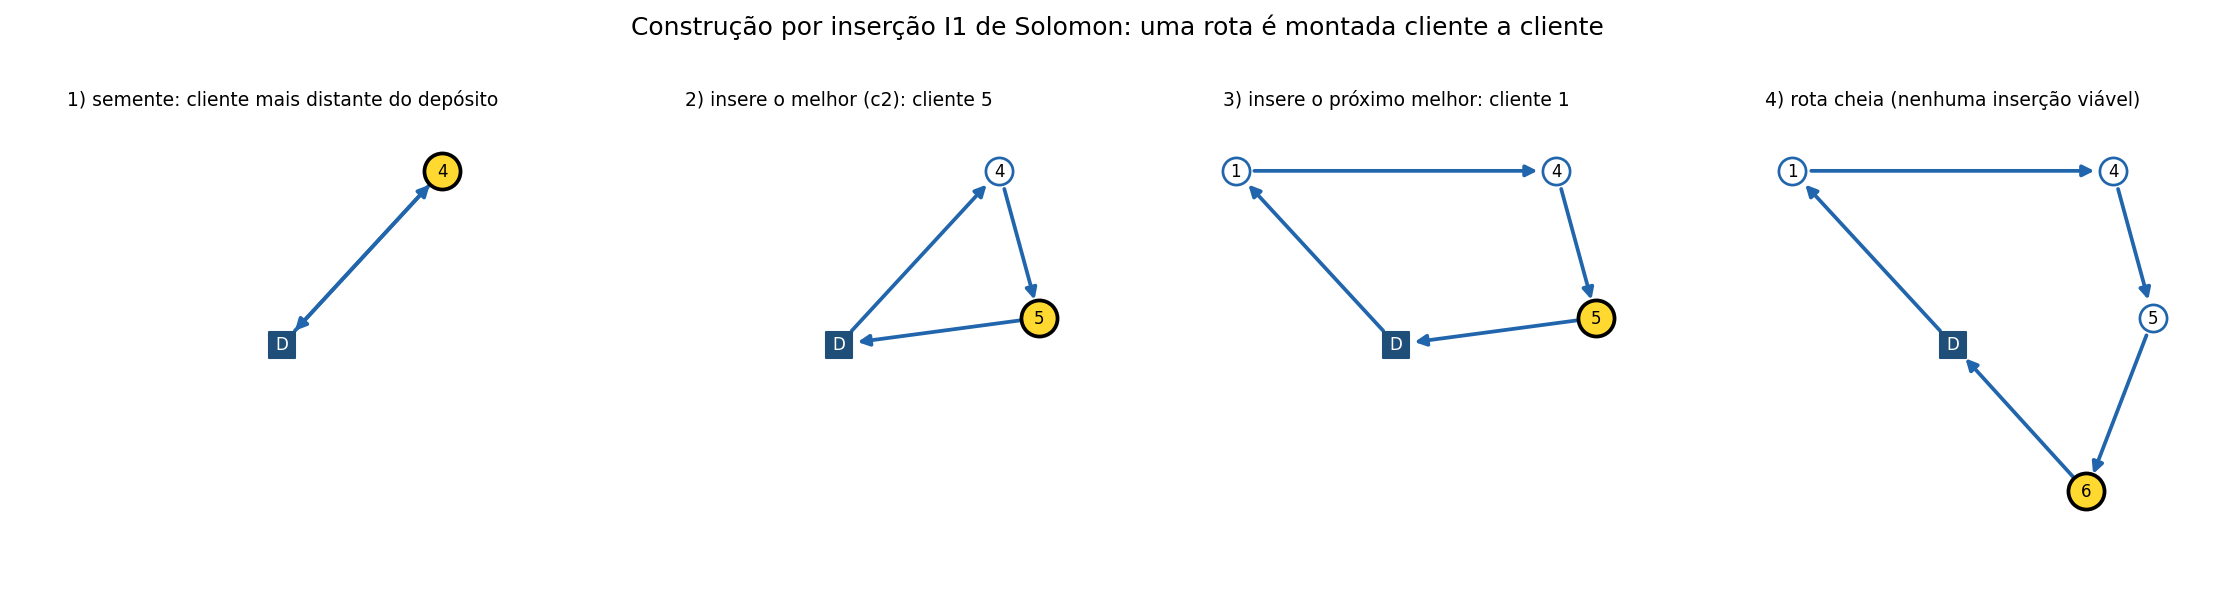
\includegraphics[width=\textwidth]{../../results/figures/construcao_i1}
\caption{Construção por inserção I1: a rota começa pela semente (cliente mais distante do depósito) e recebe, a cada passo, o cliente que maximiza $c_2$, até nenhuma inserção viável restar. O cliente recém-inserido está em amarelo.}\label{fig:i1}
\end{figure}

\subsection{Vizinhanças e sua escolha}\label{sec:vizinhancas}
Adotamos um \emph{kit} padronizado de seis operadores, compartilhado por VND, GRASP e Busca Tabu, e listado aqui na ordem em que é explorado --- complexidade computacional crescente:
\begin{itemize}[noitemsep]
\item \textbf{2-opt} (intra rota): inverte um subtrecho de uma rota;
\item \textbf{Swap} (intra e entre rotas): troca dois clientes de posição;
\item \textbf{2-opt\hspace{0.5pt}*} (entre rotas): troca as caudas de duas rotas \citep{potvin1995exchange};
\item \textbf{Relocate} (intra e entre rotas): remove um cliente e o reinsere em outra posição;
\item \textbf{Or-opt} (intra e entre rotas): move uma cadeia de 2--3 clientes, eventualmente invertida \citep{or1976traveling};
\item \textbf{Cross-exchange} (entre rotas): troca subtrechos de até 3 clientes entre duas rotas \citep{taillard1997tabu}.
\end{itemize}
Todos são operadores clássicos para o VRPTW \citep{toth2002vehicle}. Os seis cobrem os oito movimentos avaliados no relatório parcial: Relocate, Swap e Or-opt implementam as variantes \emph{intra} e \emph{entre} rotas numa única varredura, e o ``2-opt inter'' do parcial corresponde ao 2-opt\hspace{0.5pt}* de \citet{potvin1995exchange}.

\textbf{Seleção do subconjunto.} Conforme previsto no relatório parcial, os oito movimentos avaliados foram submetidos a seleção por ablação nas instâncias de treino, com Wilcoxon pareado e correção de Holm (Seção~\ref{sec:ablacao}): a remoção de qualquer operador piora o \emph{gap} médio, e nenhum subconjunto próprio supera o conjunto completo. O subconjunto selecionado é, portanto, o próprio conjunto, explorado em ordem de complexidade crescente \citep{hansen2001variable}, com a ordem derivada do custo medido de uma varredura completa.

Cada operador avalia a viabilidade do movimento por uma simulação completa da(s) rota(s) afetada(s), de modo que nenhum movimento inviável é jamais aplicado (Seção~\ref{sec:aceitacao}). A Figura~\ref{fig:operadores} ilustra o efeito de cada um.

\begin{figure}[htbp]
\centering
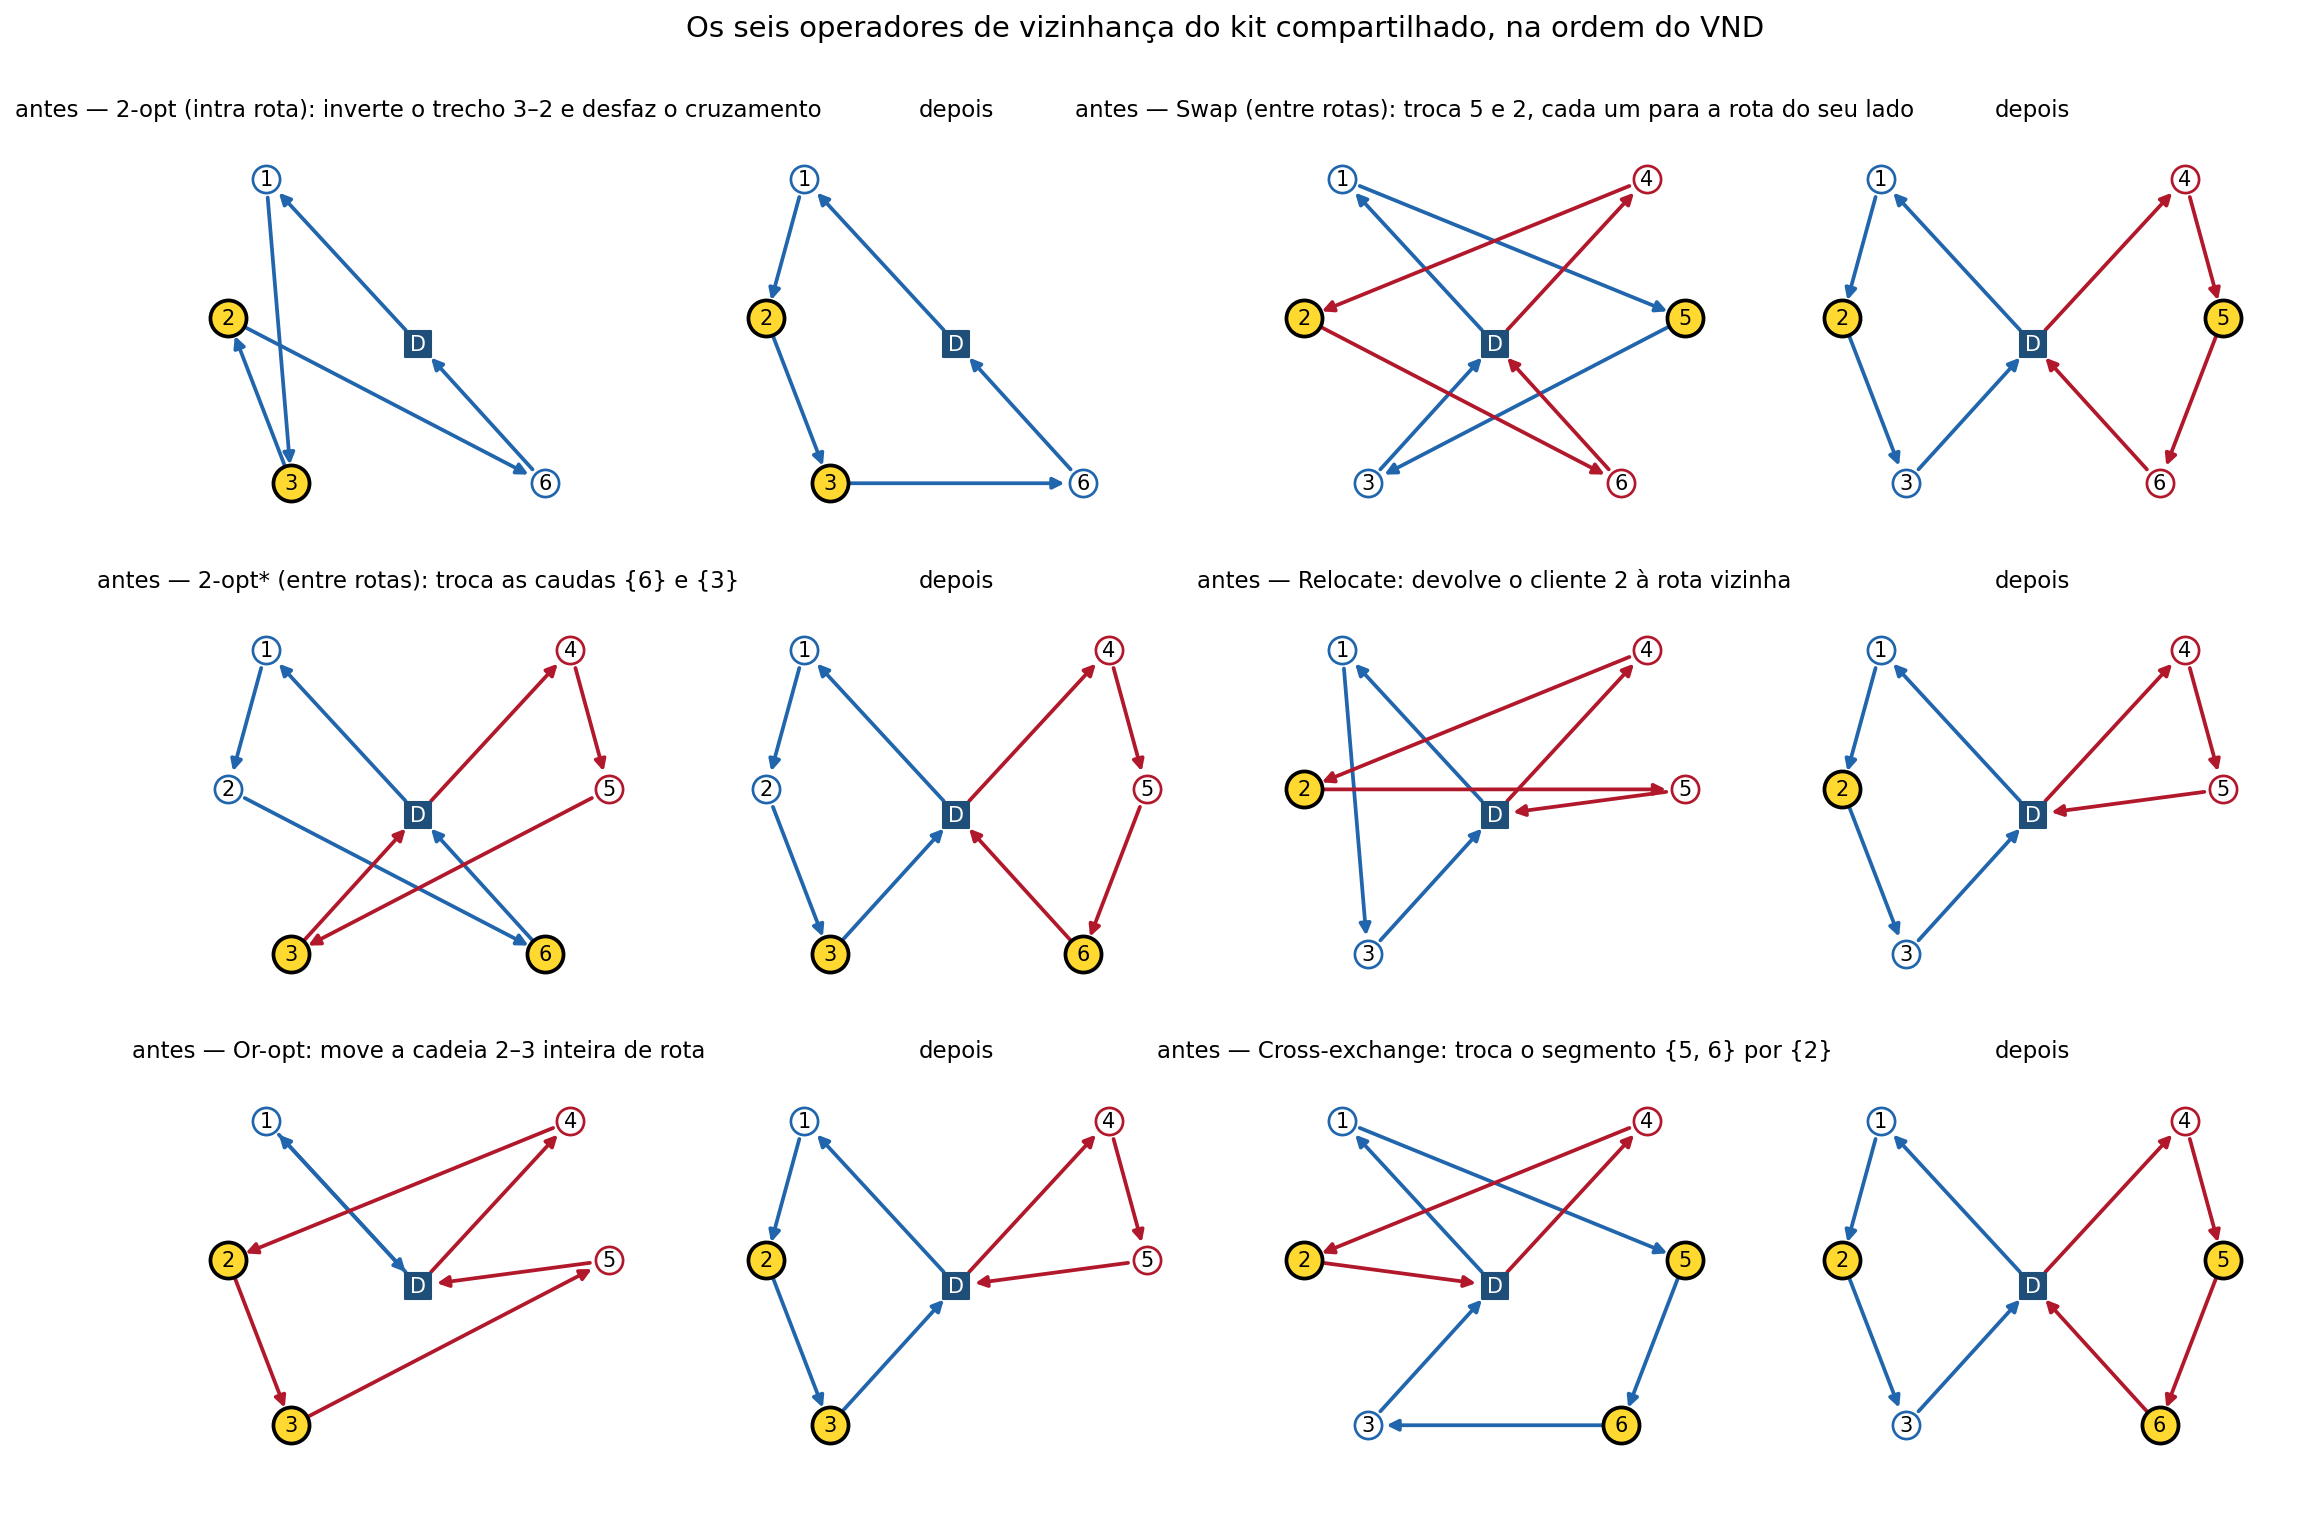
\includegraphics[width=0.6\textwidth]{../../results/figures/operadores}
\caption{Os cinco operadores de vizinhança (antes/depois), em um exemplo esquemático com duas rotas (azul e vermelha) e o depósito (D); os clientes destacados em amarelo são os que cada movimento desloca.}\label{fig:operadores}
\end{figure}

\subsection{Descida em Vizinhança Variável (VND)}\label{sec:vnd}
O VND \citep{hansen2001variable} é o primeiro método que otimiza a Equação~\eqref{eq:obj-dist} diretamente: todo movimento aceito \emph{reduz estritamente} a distância total $D(S)$, e a viabilidade é pré-condição de candidatura (Seção~\ref{sec:aceitacao}) --- de modo que a trajetória de custos é monotônica decrescente e o método para, por definição, num ótimo local. Ele percorre as vizinhanças em uma ordem fixa, \textbf{da varredura mais barata à mais cara} --- $\langle$2-opt, Swap, 2-opt\hspace{0.5pt}*, Relocate, Or-opt, Cross-exchange$\rangle$, a ordem de complexidade medida apresentada na Seção~\ref{sec:vizinhancas}. Ao encontrar uma melhora (estratégia de \emph{melhor melhora}), aplica-a e reinicia da primeira vizinhança; caso contrário, avança para a próxima. Termina em um ótimo local com relação a \emph{todas} as vizinhanças (Algoritmo~\ref{alg:vnd}). É determinístico dada a solução inicial.

\begin{algorithm}[H]
\caption{VND --- Descida em Vizinhança Variável}\label{alg:vnd}
\begin{algorithmic}[1]
\REQUIRE solução viável $S$; lista ordenada de vizinhanças $N_1,\dots,N_p$
\ENSURE ótimo local $S$ em relação a todas as vizinhanças
\STATE $\ell \gets 1$ \label{vnd:init}
\WHILE{$\ell \le p$}
  \STATE $m \gets$ melhor movimento \emph{viável e melhorante} em $N_\ell(S)$ \label{vnd:find}
  \IF{$m$ existe (reduz estritamente a distância)}
    \STATE $S \gets$ aplica $m$ a $S$;\quad $\ell \gets 1$ \label{vnd:apply}
  \ELSE
    \STATE $\ell \gets \ell + 1$ \label{vnd:next}
  \ENDIF
\ENDWHILE
\RETURN $S$
\end{algorithmic}
\end{algorithm}

\textbf{Leitura passo a passo.} O índice $\ell$ (linha~\ref{vnd:init}) aponta a vizinhança ativa. A linha~\ref{vnd:find} varre \emph{toda} a vizinhança $N_\ell$ e retorna o melhor movimento melhorante (estratégia de \emph{melhor melhora}, que escolhe o movimento de maior redução, não o primeiro encontrado --- escolha que torna a varredura independente da ordem interna de enumeração e, com isso, o resultado determinístico dado o ponto de partida). Se há ganho, a linha~\ref{vnd:apply} o aplica e \textbf{reinicia de $\ell=1$}: voltar à vizinhança mais barata após cada melhoria é o que caracteriza o VND e o que torna a descida sistemática. Sem ganho, a linha~\ref{vnd:next} passa à vizinhança seguinte; o laço encerra quando nenhuma das $p$ vizinhanças melhora $S$. A ordem por complexidade tem efeito prático direto: como cada melhoria reinicia da primeira vizinhança, os operadores de varredura barata (2-opt, Swap) absorvem a maior parte dos movimentos e reduzem o trabalho que sobra para os caros (Or-opt, Cross-exchange). É o mecanismo por trás da recomendação de \citet{hansen2001variable} de explorar primeiro a vizinhança mais simples. Em termos da \emph{formação da solução}, é aqui que a rota rígida da I1 começa a ser reorganizada: o 2-opt desfaz cruzamentos \emph{dentro} de uma rota, o 2-opt\hspace{0.5pt}* recombina as \emph{caudas} de duas rotas (podendo até fundi-las), o Relocate corrige clientes mal alocados e o Or-opt e o Cross-exchange transferem trechos \emph{entre} veículos. O ganho quantitativo sobre a I1 é apresentado na Seção~\ref{sec:comparacao}; o VND permanece, porém, preso ao primeiro ótimo local encontrado --- a limitação que motiva as meta-heurísticas a seguir.

A Figura~\ref{fig:evol} ilustra a busca local em ação: cada painel é a solução após um movimento, com a distância caindo monotonicamente até o ótimo local.

\begin{figure}[H]
\centering
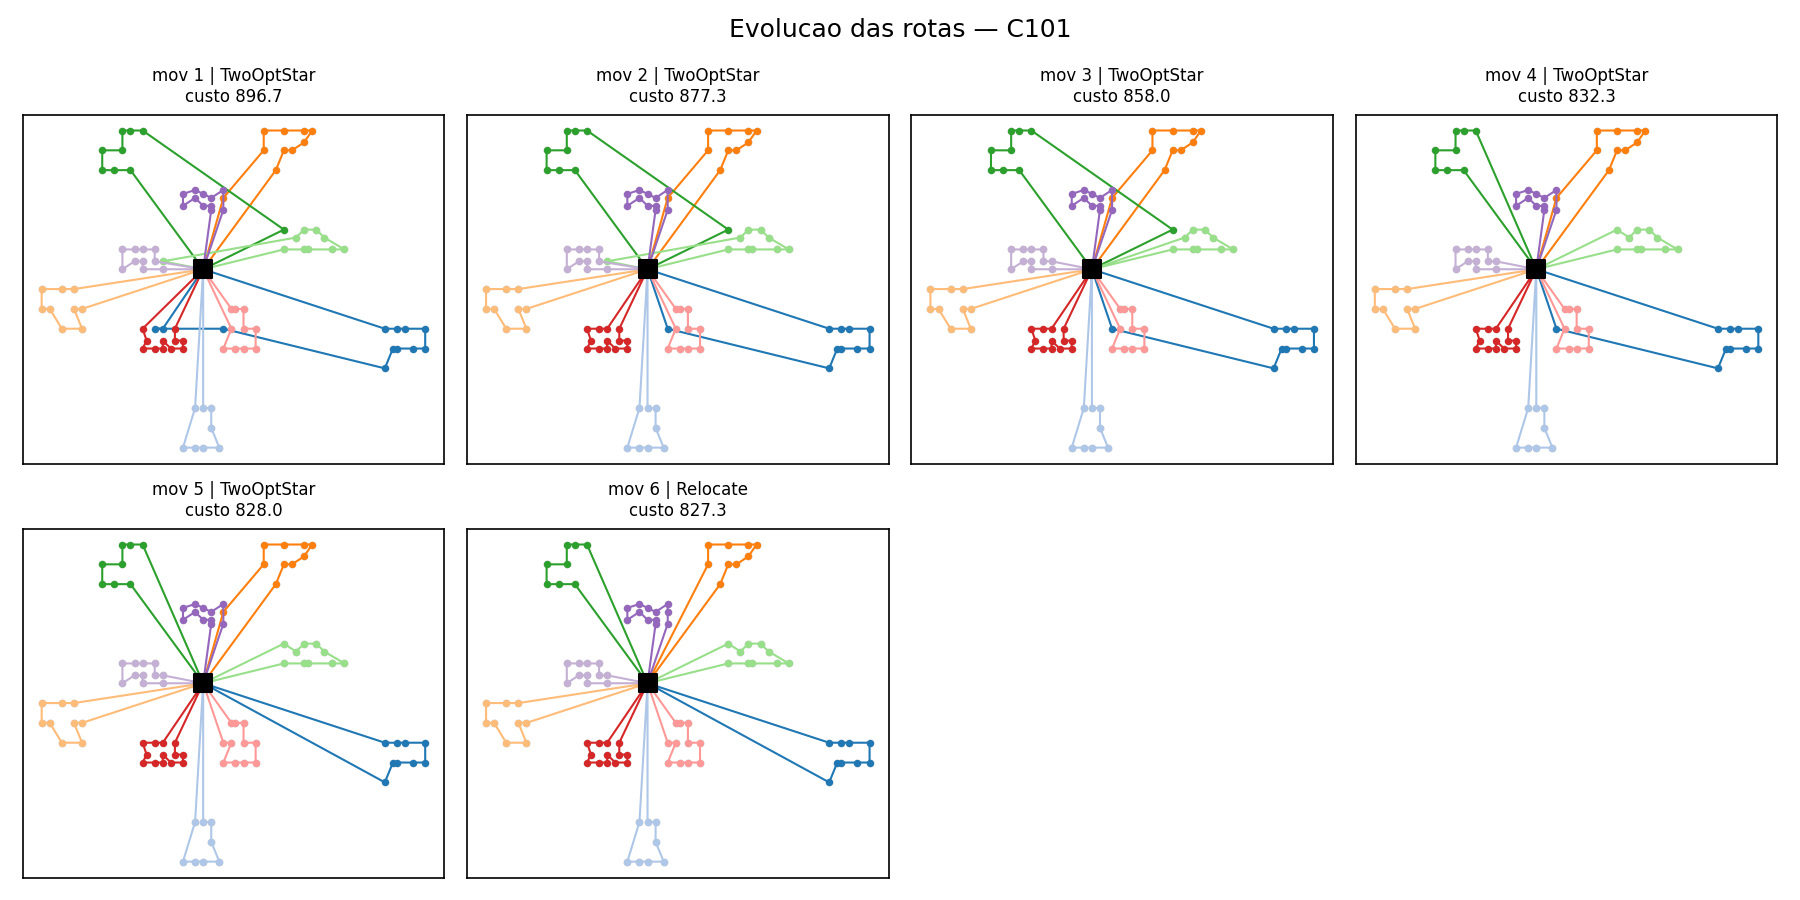
\includegraphics[width=\textwidth]{../../results/figures/evolution/evolution_C101}
\caption{Evolução das rotas na instância C101 ao longo dos movimentos da busca local (VND): cada painel mostra a solução após um movimento, com o custo decrescendo de $888{,}0$ a $827{,}3$ (o melhor conhecido).}\label{fig:evol}
\end{figure}

\subsection{GRASP}\label{sec:grasp}
O GRASP \citep{feo1995greedy,resende2003greedy} repete um ciclo \emph{construção gulosa-aleatorizada $\rightarrow$ busca local} e guarda a melhor solução. Sua função-objetivo é a mesma Equação~\eqref{eq:obj-dist}, tratada por multipartida (\emph{multi-start}): cada iteração produz um ótimo local independente e o resultado é $S^\star = \arg\min_i D(S_i)$ sobre todas as iterações --- a qualidade final é, portanto, monotonicamente não decrescente no número de iterações \citep{resende2003greedy}. A construção reusa a I1, mas substitui a escolha gulosa do melhor cliente por uma seleção aleatória dentro de uma \textbf{Lista Restrita de Candidatos} (RCL) baseada em valor: dado o conjunto de candidatos com valores $c_2$, sejam $c^{\max}$ e $c^{\min}$ o maior e o menor; a RCL contém todo candidato com
\begin{equation}
c_2(u)\ \ge\ c^{\max}-\alpha\,(c^{\max}-c^{\min}),\qquad \alpha\in[0,1].
\end{equation}
Com $\alpha=0$ recupera-se a construção gulosa; com $\alpha=1$, totalmente aleatória. A Figura~\ref{fig:rcl} ilustra a seleção. A busca local é o VND (Algoritmo~\ref{alg:vnd}). O Algoritmo~\ref{alg:grasp} resume o método; $\alpha$ é o único parâmetro, calibrado por \textit{irace}.

\begin{figure}[htbp]
\centering
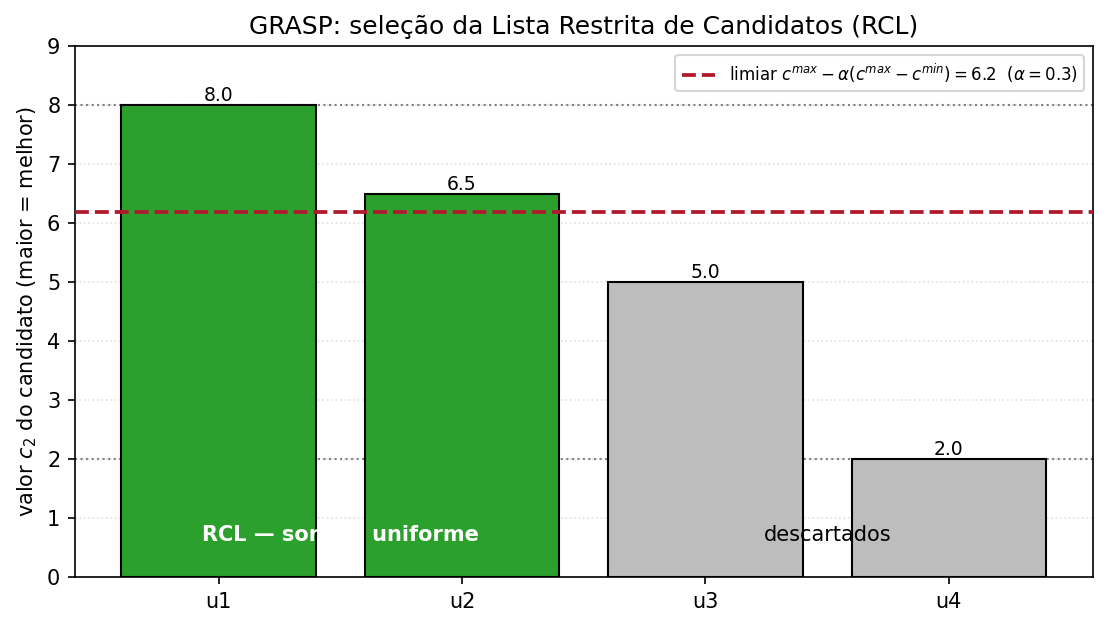
\includegraphics[width=0.72\textwidth]{../../results/figures/grasp_rcl}
\caption{Seleção da RCL no GRASP: os candidatos com $c_2$ acima do limiar $c^{\max}-\alpha(c^{\max}-c^{\min})$ (aqui $6{,}2$, com $\alpha=0{,}3$) entram na lista (verde) e um deles é sorteado uniformemente; os demais são descartados.}\label{fig:rcl}
\end{figure}

\begin{algorithm}[H]
\caption{GRASP (Feo \& Resende)}\label{alg:grasp}
\begin{algorithmic}[1]
\REQUIRE instância; parâmetro $\alpha$; orçamento $K$ (iterações sem melhora)
\ENSURE melhor solução $S^\star$
\STATE $S^\star \gets$ I1 \COMMENT{partida comum a todos os métodos (Seção~\ref{sec:i1})};\quad $k \gets 0$ \label{g:init}
\WHILE{critério de parada não satisfeito}
  \STATE $S \gets$ \textsc{ConstruçãoGulosa-Aleatorizada}($\alpha$) \label{g:build}
  \STATE $S \gets$ \textsc{VND}($S$) \label{g:ls}
  \IF{distância$(S) <$ distância$(S^\star)$}
    \STATE $S^\star \gets S$;\quad $k \gets 0$ \label{g:improve}
  \ELSE
    \STATE $k \gets k+1$ \label{g:noimprove}
  \ENDIF
  \IF{$k \ge K$}
    \STATE \textbf{interrompa} \label{g:stop}
  \ENDIF
\ENDWHILE
\RETURN $S^\star$
\end{algorithmic}
\end{algorithm}

\textbf{Leitura passo a passo.} A linha~\ref{g:init} difere da forma de livro-texto (que parte de incumbente vazio) em um ponto deliberado: o \emph{incumbente} --- a melhor solução encontrada até o momento, que será devolvida ao final --- é inicializado com a solução da I1 pura, a mesma partida entregue ao VND e à Busca Tabu. Com isso, o resultado do GRASP nunca é pior que a I1 por garantia, e não por observação empírica --- e a comparação entre os métodos parte do mesmo ponto. Cada iteração é então um ciclo \emph{construção $\rightarrow$ busca local}: a linha~\ref{g:build} gera uma solução nova com aleatorização controlada por $\alpha$ (a RCL da Figura~\ref{fig:rcl}), e a linha~\ref{g:ls} a conduz a um ótimo local pelo VND (Algoritmo~\ref{alg:vnd}). A aleatorização age apenas na escolha de qual cliente inserir; a regra de semente e o critério $c_2$ permanecem os da I1, e é por isso que, com $\alpha=0$, o GRASP reproduz a I1 exatamente --- propriedade verificada por teste automatizado nas 56 instâncias. A linha~\ref{g:improve} retém a melhor solução já vista e zera o contador de estagnação; a linha~\ref{g:noimprove} o incrementa quando não há ganho; e a linha~\ref{g:stop} encerra após $K$ iterações sem melhora. O que o GRASP acrescenta à formação da solução é \emph{diversificação estruturada}: ao reconstruir a rota do zero a cada iteração, ele rompe a dependência da semente única da I1 --- cada RCL produz uma topologia de rotas diferente ---, e o resultado final é a melhor entre centenas de descidas independentes (Seção~\ref{sec:comparacao}).

\subsection{GRASP Reativo}\label{sec:rgrasp}
O GRASP Reativo \citep{prais2000reactive} otimiza a mesma função-objetivo do GRASP --- Equação~\eqref{eq:obj-dist}, por multi-partida --- diferindo apenas em \emph{como} o parâmetro de aleatorização é escolhido: em vez de um $\alpha$ fixo, mantém-se um conjunto discreto $\{\alpha_1,\dots,\alpha_g\}$ (grade $0{,}05,0{,}10,\dots,0{,}50$) com probabilidades $p_i$ de seleção. A cada bloco de \textit{block} iterações, as probabilidades são atualizadas de modo que valores de $\alpha$ que produziram soluções melhores fiquem mais prováveis --- o expoente $\delta$ regula a agressividade desse aprendizado ($\delta$ baixo mantém as probabilidades próximas do uniforme; $\delta$ alto concentra rapidamente no melhor $\alpha$):
\begin{equation}
q_i=\left(\frac{Z^\star}{\bar Z_i}\right)^{\!\delta},\qquad p_i=\frac{q_i}{\sum_{j} q_j},
\end{equation}
onde $Z^\star$ é o melhor custo encontrado e $\bar Z_i$ o custo médio (acumulado ao longo de toda a execução) das soluções obtidas com $\alpha_i$. Os parâmetros $\delta$ (expoente) e \textit{block} são calibrados por \textit{irace}. O Algoritmo~\ref{alg:rgrasp} detalha o método; nas primeiras $g$ iterações cada $\alpha$ é experimentado uma vez (\emph{aquecimento}) antes de a amostragem por probabilidade começar.

\begin{algorithm}[H]
\caption{GRASP Reativo (Prais \& Ribeiro)}\label{alg:rgrasp}
\begin{algorithmic}[1]
\REQUIRE grade $\{\alpha_1,\dots,\alpha_g\}$; expoente $\delta$; tamanho de bloco \textit{block}; orçamento $K$
\ENSURE melhor solução $S^\star$
\STATE $p_i \gets 1/g$,\ $\Sigma_i \gets 0$,\ $n_i \gets 0$ \textbf{para todo} $i$;\quad $S^\star \gets$ I1;\quad $k \gets 0$;\quad $\mathit{it} \gets 0$ \label{rg:init}
\WHILE{critério de parada não satisfeito}
  \IF{$\mathit{it} < g$}
    \STATE $j \gets \mathit{it}+1$ \COMMENT{aquecimento: cada $\alpha$ uma vez} \label{rg:warm}
  \ELSE
    \STATE $j \gets$ amostra de $\{1,\dots,g\}$ segundo as probabilidades $p$ \label{rg:sample}
  \ENDIF
  \STATE $S \gets$ \textsc{VND}\big(\textsc{ConstruçãoGulosa-Aleatorizada}($\alpha_j$)\big) \label{rg:build}
  \STATE $c \gets$ distância$(S)$;\quad $\Sigma_j \gets \Sigma_j + c$;\quad $n_j \gets n_j + 1$ \label{rg:acc}
  \IF{$c <$ distância$(S^\star)$}
    \STATE $S^\star \gets S$;\quad $k \gets 0$ \label{rg:improve}
  \ELSE
    \STATE $k \gets k+1$
  \ENDIF
  \STATE $\mathit{it} \gets \mathit{it}+1$
  \IF{$k \ge K$}
    \STATE \textbf{interrompa}
  \ENDIF
  \IF{$\mathit{it} \bmod \textit{block} = 0$}
    \STATE para todo $i$ com $n_i>0$:\ $\bar Z_i \gets \Sigma_i/n_i$,\ \ $q_i \gets (Z^\star/\bar Z_i)^\delta$ \label{rg:q}
    \STATE $p_i \gets q_i / \sum_l q_l$ \textbf{para todo} $i$ \label{rg:p}
  \ENDIF
\ENDWHILE
\RETURN $S^\star$
\end{algorithmic}
\end{algorithm}

\textbf{Leitura passo a passo.} O reativo difere do GRASP por \emph{aprender} qual $\alpha$ funciona melhor em cada instância. As linhas~\ref{rg:warm}--\ref{rg:sample} escolhem o $\alpha$: nas primeiras $g$ iterações cada valor é testado uma vez (aquecimento, para que nenhum $\alpha$ comece com vantagem espúria); depois, $\alpha$ é sorteado conforme as probabilidades $p$. A linha~\ref{rg:acc} acumula o custo médio obtido por cada $\alpha$ e, a cada \textit{block} iterações, as linhas~\ref{rg:q}--\ref{rg:p} recalculam as probabilidades pela razão $q_i=(Z^\star/\bar Z_i)^\delta$ --- valores de $\alpha$ que produziram soluções melhores tornam-se mais prováveis. Na formação da solução, isso ajusta automaticamente o equilíbrio guloso$\leftrightarrow$aleatório ao perfil da instância; se esse aprendizado se traduz em vantagem mensurável sobre o GRASP de $\alpha$ fixo é uma pergunta empírica, respondida pela análise estatística da Seção~\ref{sec:comparacao}.

\subsection{Busca Tabu}\label{sec:tabu}
Adotamos a forma clássica e mais simples da Busca Tabu \citep{glover1989tabu,glover1990tabu}: a cada iteração, move-se para o \emph{melhor vizinho admissível} sobre o kit de vizinhanças, aceitando, se necessário, movimentos que pioram a solução, para escapar de ótimos locais. A função-objetivo é a mesma Equação~\eqref{eq:obj-dist}, com uma distinção operacional: a solução \emph{corrente} pode piorar de um passo para o outro; quem realiza a minimização é o \emph{incumbente} $S^\star$, que retém o menor $D(S)$ visitado ao longo da trajetória única do método. Um movimento é \emph{tabu} se algum cliente que ele toca foi movido nas últimas \textit{tenure} iterações, a menos que satisfaça o critério de \emph{aspiração por objetivo} (produzir um novo melhor global). Adota-se também a \emph{aspiração por omissão} \citep{glover1997tabu}: se \textbf{todos} os movimentos disponíveis estiverem tabu, revoga-se o status do grupo de clientes com prazo de expiração mais próximo e a varredura é refeita, em vez de encerrar a busca --- sem ela, a lista tabu pode esgotar a vizinhança e truncar a execução muito antes do critério de parada. O atributo tabu é o cliente movido; é uma simplificação deliberada (em vez do arco/atributo de movimento), mantida para preservar a forma ``de livro-texto''. Não há religação de caminhos, intensificação ou diversificação por frequência. O único parâmetro é \textit{tenure}, calibrado por \textit{irace} (Algoritmo~\ref{alg:tabu}).

\begin{algorithm}[H]
\caption{Busca Tabu (Glover, forma clássica)}\label{alg:tabu}
\begin{algorithmic}[1]
\REQUIRE solução inicial $S$ (da I1); \textit{tenure}; orçamento $K$
\ENSURE melhor solução $S^\star$
\STATE $S^\star \gets S$;\quad $k \gets 0$ \label{t:init}
\WHILE{critério de parada não satisfeito}
  \STATE $m \gets$ melhor movimento \emph{viável} e \emph{admissível} em $N(S)$ \COMMENT{não-tabu, ou tabu com aspiração} \label{t:find}
  \IF{não existe movimento admissível}
    \STATE revogue o status tabu do grupo com menor prazo de expiração; \textbf{refaça a varredura} \COMMENT{aspiração por omissão} \label{t:default}
  \ENDIF
  \STATE $S \gets$ aplica $m$ a $S$; marque o(s) cliente(s)-atributo de $m$ como tabu por \textit{tenure} iterações \label{t:apply}
  \IF{distância$(S) <$ distância$(S^\star)$}
    \STATE $S^\star \gets S$;\quad $k \gets 0$ \label{t:improve}
  \ELSE
    \STATE $k \gets k+1$ \label{t:noimprove}
  \ENDIF
  \IF{$k \ge K$}
    \STATE \textbf{interrompa}
  \ENDIF
\ENDWHILE
\RETURN $S^\star$
\end{algorithmic}
\end{algorithm}

\textbf{Leitura passo a passo.} A cada iteração, a linha~\ref{t:find} varre todo o kit de vizinhanças e escolhe o melhor movimento \emph{admissível} --- não-tabu ou, se tabu, que satisfaça a aspiração por objetivo. Diferentemente do VND, a Tabu \textbf{não} exige que o movimento melhore: a linha~\ref{t:apply} pode aplicar uma piora controlada, e é assim que a busca escapa de ótimos locais. O movimento torna tabu, por \textit{tenure} iterações, o(s) cliente(s) que ele toca (memória de curto prazo), o que impede a busca de reverter movimentos recentes e ciclar. O \textit{tenure} regula o compromisso central do método: valores pequenos liberam os clientes cedo e intensificam a busca na região atual; valores grandes prolongam as proibições e forçam a exploração de regiões novas. Quando a lista tabu chega a bloquear \emph{todos} os movimentos --- situação comum com \textit{tenure} alto em instâncias pequenas ---, a linha~\ref{t:default} aplica a aspiração por omissão: expira o grupo de proibições mais antigo e repete a varredura, sem consumir iteração; a busca só termina pelo critério de parada. A linha~\ref{t:improve} guarda o melhor já visto. Na formação da solução, a Tabu percorre uma \emph{única} trajetória contínua, refinando a estrutura herdada da I1 sem reinícios --- em contraste com o GRASP, que explora múltiplas estruturas independentes; a comparação quantitativa está na Seção~\ref{sec:comparacao}.

\subsection{Critérios de aceitação}\label{sec:aceitacao}
Os cinco métodos diferem essencialmente em \emph{o que aceitam} a cada passo. Tornamos isso explícito:
\begin{itemize}[noitemsep]
\item \textbf{Filtro de viabilidade (comum a todos).} Um movimento só é \emph{candidato} se a(s) rota(s) resultante(s) satisfaz(em) a Equação~\eqref{eq:viab}. Movimentos inviáveis são descartados \emph{antes} da comparação de custo. Esse filtro é o que garante o invariante da Seção~\ref{sec:invariantes}.
\item \textbf{VND e GRASP:} aceitam um movimento apenas se ele \emph{reduz estritamente} a distância (melhora). O GRASP, além disso, guarda a melhor solução ao longo das reinicializações.
\item \textbf{Busca Tabu:} aceita, a cada iteração, o \emph{melhor vizinho admissível}, mesmo que piore a solução corrente; a regra tabu proíbe reverter movimentos recentes (memória de curto prazo), e a aspiração libera um movimento tabu se ele gerar um novo melhor global.
\item \textbf{RCL (GRASP):} na construção, um candidato é aceito na lista restrita se seu valor $c_2$ está dentro de uma fração $\alpha$ do intervalo $[c^{\min},c^{\max}]$; a escolha final é uniforme sobre a RCL.
\end{itemize}

\subsection{Exemplos ilustrativos do funcionamento}\label{sec:exemplos}
Para tornar concretos os mecanismos centrais, apresentamos três exemplos mínimos e verificáveis.

\textbf{(a) Critério Push Forward (viabilidade de inserção em $O(1)$).} Considere o depósito $D=(0,0)$, horizonte $[0,100]$, e a rota $\langle D, A, B, D\rangle$ com $A=(10,0)$, janela $[5,40]$, serviço $5$; $B=(30,0)$, janela $[20,60]$, serviço $5$; capacidade $Q=50$ e demandas $10$. As distâncias são $d_{DA}=10$, $d_{AB}=20$, $d_{BD}=30$. A Tabela~\ref{tab:pf} mostra o cronograma: partindo de $D$ em $t=0$, todos os inícios respeitam as janelas e o retorno ocorre em $70\le 100$. A \emph{folga} (\textit{slack}) de cada cliente é a margem de adiamento do seu início sem violar nada à frente: $\mathrm{slack}(B)=\min(60-35,\,100-70)=25$ e $\mathrm{slack}(A)=\min(40-10,\,0+25)=25$.

\begin{table}[H]
\centering
\caption{Cronograma da rota $\langle D,A,B,D\rangle$ do exemplo (a).}\label{tab:pf}
\begin{tabular}{lcccc}
\toprule
nó & chegada & início & partida & janela \\
\midrule
$A$ & $10$ & $10$ & $15$ & $[5,40]$ \\
$B$ & $35$ & $35$ & $40$ & $[20,60]$ \\
$D$ (retorno) & $70$ & --- & --- & $[0,100]$ \\
\bottomrule
\end{tabular}
\end{table}

Suponha inserir $C=(15,0)$, janela $[10,50]$, serviço $5$, demanda $10$, entre $A$ e $B$. Verifica-se em $O(1)$: a capacidade ($20+10\le 50$); o início de $C$, $\max(15+5,10)=20\le 50$; e o novo início de $B$, $\max(25+15,20)=40$, um \emph{deslocamento} de $40-35=5$. Como $5\le \mathrm{slack}(B)=25$, a inserção é \textbf{viável} --- sem reavaliar a rota inteira. É exatamente esse teste que cada operador de melhoria aplica antes de aceitar um movimento.

\textbf{(b) Lista Restrita de Candidatos (GRASP).} Suponha quatro candidatos com valores $c_2$: $u_1{=}8{,}0$, $u_2{=}6{,}5$, $u_3{=}5{,}0$, $u_4{=}2{,}0$, logo $c^{\max}{=}8{,}0$ e $c^{\min}{=}2{,}0$. Com $\alpha=0{,}3$, o limiar é $8{,}0-0{,}3\cdot(8{,}0-2{,}0)=6{,}2$; assim $\mathrm{RCL}=\{u_1,u_2\}$ e o próximo cliente é sorteado uniformemente entre os dois. Com $\alpha=0$ a RCL seria $\{u_1\}$ (guloso puro); com $\alpha=1$ conteria todos (aleatório puro). É esse parâmetro que regula o equilíbrio guloso--aleatório, calibrado por \textit{irace}.

\textbf{(c) Uma iteração da Busca Tabu.} Da solução corrente, a varredura encontra como melhor movimento \emph{viável e admissível} um Relocate do cliente $7$, com variação de distância $\Delta=-3{,}1$. Aplica-se o movimento e o cliente $7$ torna-se \emph{tabu} por \textit{tenure} iterações: nesse período, qualquer movimento que toque o cliente $7$ é proibido --- \emph{exceto} se produzir um custo melhor que o melhor global já visto (aspiração). Assim, a busca aceita pioras controladas para escapar de ótimos locais, mas evita ciclar revertendo movimentos recentes.

\subsection{Parametrização}\label{sec:parametrizacao}
Cada parâmetro deste estudo pertence a uma de três categorias, e a categoria determina como seu valor foi obtido. Parâmetros \textbf{fixos} definem o terreno comum da comparação --- a solução inicial, o conjunto de vizinhanças, a convenção de distância --- e por isso não podem ser ajustados por método: calibrá-los daria a um algoritmo uma condição de partida diferente da dos demais. Parâmetros \textbf{calibrados} são os de qualidade intrínsecos a cada meta-heurística, ajustados pelo \textit{irace} sobre as instâncias de treino (Seção~\ref{sec:calibracao}); seus valores finais ficam registrados em \texttt{experiments/config/tuned.json} e não são transcritos à mão para este texto. Parâmetros \textbf{declarados} são orçamentos computacionais, para os quais não existe valor ótimo a descobrir (Seção~\ref{sec:parada}). A Tabela~\ref{tab:parametros} consolida as três categorias.

\begin{table}[H]
\centering
\caption{Parâmetros dos algoritmos: papel, valor ou intervalo de busca, e origem de cada um.}\label{tab:parametros}
\begin{tabular}{llllc}
\toprule
\textbf{Algoritmo} & \textbf{Parâmetro} & \textbf{Papel} & \textbf{Valor / intervalo} & \textbf{Origem} \\
\midrule
I1        & $\mu$              & economia do arco removido em $c_{11}$        & $1{,}0$            & fixo \\
I1        & $\lambda$          & peso da distância ao depósito em $c_2$       & $2{,}0$            & fixo \\
I1        & $\alpha_1,\alpha_2$& mistura distância$\times$tempo em $c_1$      & $1{,}0$ / $0{,}0$  & fixo \\
I1        & semente            & cliente que abre cada rota                   & mais distante      & fixo \\
VND       & ordem              & sequência de exploração das vizinhanças     & complexidade medida & fixo \\
GRASP     & $\alpha$           & largura da RCL (guloso$\leftrightarrow$aleatório) & $(0;\ 0{,}5)$ & calibrado \\
Reativo   & $\delta$           & expoente da reponderação das probabilidades  & $(0{,}5;\ 3{,}0)$  & calibrado \\
Reativo   & \textit{block\_frac} & cadência de reponderação, fração de $K$    & $(0{,}02;\ 0{,}40)$ & calibrado \\
Reativo   & grade de $\alpha$  & valores candidatos ao sorteio                & $0{,}05$--$0{,}50$ (10) & fixo \\
Tabu      & \textit{tenure}    & duração da proibição (memória curta)         & $(5;\ 80)$         & calibrado \\
todos     & $K$                & iterações sem melhoria (parada)              & $800$              & declarado \\
todos     & teto de tempo      & salvaguarda de execução                      & $600$ s            & declarado \\
\bottomrule
\end{tabular}
\end{table}

Quatro escolhas da tabela merecem justificativa explícita. Os parâmetros da I1 usam a configuração de distância de \citet{solomon1987algorithms} ($\alpha_2=0$), coerente com o objetivo DIMACS, e são fixos porque a I1 é a partida comum de todos os métodos. O intervalo de $\alpha$ do GRASP para em $0{,}5$ porque, acima disso, a construção degenera em sorteio quase uniforme e perde a estrutura da I1 que a busca local aproveita. O \textit{block\_frac} do Reativo é expresso como fração de $K$, e não em iterações absolutas, para que o número de reponderações independa do orçamento --- com bloco absoluto, um orçamento pequeno pode encerrar a execução antes da primeira reponderação, e o mecanismo reativo simplesmente não opera. O teto do \textit{tenure} foi definido após uma primeira rodada de calibração em que o vencedor caiu na fronteira superior do intervalo então vigente; um vencedor de fronteira indica intervalo curto, e a resposta metodológica é alargá-lo e repetir a corrida, não reportar o valor de borda como ótimo.

\subsection{Critério de parada}\label{sec:parada}
A I1 e o VND são determinísticos e terminam naturalmente (a I1 quando todos os clientes estão roteados; o VND em um ótimo local). Para as meta-heurísticas estocásticas/iterativas (GRASP, GRASP Reativo e Busca Tabu) adotamos como critério primário o \textbf{número de iterações consecutivas sem melhora do incumbente} ($K$), na unidade natural de iteração de cada método (uma iteração do GRASP é uma construção seguida de VND; uma iteração da Tabu é um movimento). O tempo de relógio é registrado e reportado, mas serve apenas como teto de segurança. Essa escolha favorece a \textbf{reprodutibilidade} (uma parada por tempo depende da máquina), ao custo de que uma ``iteração'' não representa o mesmo esforço entre métodos; por isso reportamos também o tempo e o número de iterações de cada execução, e as curvas tempo-alvo (TTT), tornando o esforço transparente. Observa-se que a \emph{competição} DIMACS em si pontua por tempo de relógio padronizado e integral primal \citep{dimacs12vrptw}; como este trabalho é um \emph{estudo comparativo} (não uma submissão à competição), adotar a parada por iterações sem melhoria é uma opção metodológica deliberada em favor da reprodutibilidade, mantendo a mesma convenção de distância e objetivo do desafio.

\subsection{Calibração de parâmetros (irace)}\label{sec:calibracao}
A calibração é feita com o pacote \textit{irace} \citep{lopez2016irace}, padrão de fato para configuração automática de algoritmos. Seu mecanismo é a \emph{corrida} (\textit{racing}): as configurações candidatas são avaliadas instância a instância e, a cada rodada, um teste estatístico elimina as que já se mostram inferiores --- concentrando o orçamento de avaliações nas candidatas sobreviventes, em vez de gastá-lo uniformemente. Para evitar superajuste, as 56 instâncias são divididas em \textbf{treino} (28) e \textbf{teste} (28), estratificadas por família (C/R/RC) e tipo (1/2); o \textit{irace} usa apenas o treino, e os resultados são reportados no teste e no conjunto completo. Adotamos um desenho \textbf{desacoplado}: o critério de parada $K$ é \emph{declarado} (a seguir), e o \textit{irace} calibra \emph{apenas} os hiperparâmetros de qualidade de cada método --- GRASP: $\alpha$; Reativo: $\delta$ e \textit{block\_frac}; Tabu: \textit{tenure}. Os demais elementos (parâmetros da I1, conjunto de vizinhanças, número de execuções) são \emph{fixados} por justiça. A função-objetivo do \textit{irace} é o \emph{gap} de distância ao melhor valor conhecido, que normaliza escalas entre instâncias. A justificativa de cada faixa de busca e da separação ``calibrar vs.\ fixar'' está documentada no arquivo \texttt{TUNING\_RATIONALE}.

\textbf{Fixação de $K$.} O critério de parada $K$ é um \emph{orçamento}, não um parâmetro de qualidade: mais iterações sem melhora nunca pioram o gap. Essa monotonicidade tem uma consequência que precisa ser enunciada, porque ela decide o procedimento: \textbf{não existe valor ótimo de $K$ a ser descoberto}. Um orçamento monótono não pode ser escolhido minimizando o objetivo --- calibrá-lo pelo gap, junto aos parâmetros de qualidade, o levaria sempre ao teto do intervalo de busca, conflacionando \emph{orçamento} e \emph{qualidade}. É também o motivo pelo qual a literatura de GRASP e de Busca Tabu não deriva $K$: ela o \emph{declara} \citep{feo1995greedy,resende2003greedy,prais2000reactive}.

Adotamos, portanto, $K$ como \textbf{orçamento computacional declarado}, \emph{uniforme entre os métodos} --- $K_{\mathrm{GRASP}} = K_{\mathrm{Reativo}} = K_{\mathrm{Tabu}} = \Kgrasp$ --- de modo que a regra de parada seja a mesma para todos. A Tabela~\ref{tab:orcamento} mostra, nas instâncias de treino, o que cada orçamento entrega e o que custa. Em $K=800$ a execução mediana leva $15{,}6$~s no GRASP, $22{,}7$~s no Reativo e $6{,}8$~s na Busca Tabu, com pior caso de $76$~s --- com ampla margem em relação ao teto de segurança de $600$~s. Dobrar o orçamento para $K=1600$ reduz o gap do GRASP em $0{,}19$ ponto percentual e custa $1{,}8\times$ mais tempo ($2{,}3\times$ no Reativo).

A escolha não influencia nenhuma conclusão do estudo, e isso é verificado e não suposto: \textbf{o ordenamento dos métodos e o resultado dos testes par a par são idênticos em toda a faixa medida}, de $K=50$ a $K=3200$ --- uma variação de $64\times$ (Apêndice~\ref{ap:orcamento}). A contrapartida de um $K$ uniforme é que uma ``iteração'' não custa o mesmo em cada método; por isso reportamos o tempo, o número de iterações e as curvas tempo-alvo (TTT), e complementamos a leitura com a comparação sob tempo igual e o integral primal.

\begin{table}[htbp]
\centering
\caption{Efeito do orçamento de parada. \emph{Gap}: distância percentual média ao melhor valor conhecido, nas 28 instâncias de treino. \emph{Tempo}: mediana por execução, medida sem concorrência em seis instâncias-amostra (uma por família e tipo). O valor adotado ($K=800$) está em negrito. O gap decresce ao longo de toda a faixa medida, sem platô --- razão pela qual $K$ é declarado como orçamento computacional, e não derivado de um ponto de convergência.}\label{tab:orcamento}
\begin{tabular}{r rrr rrr}
\toprule
& \multicolumn{3}{c}{\emph{gap} médio (\%)} & \multicolumn{3}{c}{tempo mediano (s)} \\
\cmidrule(lr){2-4}\cmidrule(lr){5-7}
$K$ & GRASP & Reativo & Tabu & GRASP & Reativo & Tabu \\
\midrule
50 & 3{,}49 & 3{,}11 & 5{,}99 & --- & --- & --- \\
100 & 3{,}15 & 2{,}71 & 5{,}47 & --- & --- & --- \\
200 & 2{,}39 & 2{,}27 & 4{,}68 & 4{,}6 & 6{,}9 & 1{,}6 \\
400 & 2{,}17 & 1{,}93 & 4{,}28 & 9{,}5 & 11{,}8 & 3{,}9 \\
800 & \textbf{1{,}86} & \textbf{1{,}65} & \textbf{4{,}04} & \textbf{15{,}6} & \textbf{22{,}7} & \textbf{6{,}8} \\
1600 & 1{,}67 & 1{,}52 & 3{,}64 & 27{,}9 & 52{,}5 & 13{,}9 \\
3200 & 1{,}47 & 1{,}20 & 3{,}28 & --- & --- & --- \\
\bottomrule
\end{tabular}
\end{table}


\subsection{Comparação estatística}\label{sec:estatistica}
Cada algoritmo estocástico é executado 30 vezes por instância, com sementes independentes registradas --- tamanho de amostra usual em comparações de meta-heurísticas, suficiente para estimativas estáveis de média e dispersão por instância; os determinísticos (I1, VND, Busca Tabu) executam uma vez, por não possuírem fonte de aleatoriedade. Para comparar os métodos sobre as 56 instâncias usamos o teste não-paramétrico de \textbf{Friedman} sobre os \emph{ranks} por instância: em cada instância, os $k$ métodos são ordenados do menor ao maior gap médio, e o \emph{rank} de um método é sua posição nessa ordenação ($1$ = melhor; empates recebem a média das posições). O teste pergunta se os ranks médios diferem mais do que o acaso explicaria, e é seguido do pós-teste de \textbf{Nemenyi} (todas as comparações par a par), conforme \citet{demsar2006statistical}. A estatística de Friedman, \emph{com correção para empates} (frequentes, pois na família C vários métodos atingem o ótimo), é
\begin{equation}
\chi^2_F=\frac{1}{C}\cdot\frac{12N}{k(k+1)}\left[\sum_{j=1}^{k}R_j^2-\frac{k(k+1)^2}{4}\right],
\qquad C=1-\frac{\sum_g (t_g^3-t_g)}{N\,(k^3-k)},
\end{equation}
com $N$ instâncias, $k$ algoritmos, $R_j$ o \emph{rank} médio do algoritmo $j$ (rank $1$ = melhor) e $t_g$ o tamanho de cada grupo de empate. A correção para empates é relevante neste conjunto: na família C vários métodos atingem o mesmo custo, e ignorá-la subestimaria a estatística. É o cálculo realizado pela implementação (\texttt{scipy.stats.friedmanchisquare}). No pós-teste de Nemenyi, dois algoritmos diferem significativamente se seus ranks médios distam mais que a \emph{diferença crítica}
\begin{equation}
CD=q_\alpha\sqrt{\frac{k(k+1)}{6N}},
\end{equation}
onde $q_\alpha$ é o valor crítico do \emph{range} estudentizado (dividido por $\sqrt2$); para $k=5$ e $\alpha=0{,}05$ ($q_\alpha=2{,}728$), tem-se $CD=0{,}815$ com $N=56$. Os resultados são sintetizados em um \emph{diagrama de diferença crítica} (CD). O teste de Friedman é apropriado por ser pareado (mesmas instâncias para todos os métodos) e robusto a distribuições não-normais dos gaps.

O pós-teste de Nemenyi opera sobre \emph{ranks médios}, e uma limitação conhecida dessa família de procedimentos é que a conclusão sobre um par de métodos depende também do desempenho dos demais métodos incluídos na comparação \citep{benavoli2016should}. Por isso, cada comparação par a par de interesse é adicionalmente examinada pelo teste de \textbf{Wilcoxon pareado} sobre os gaps por instância, com correção de \textbf{Holm} para as múltiplas comparações \citep{garcia2008extension} --- um procedimento que usa apenas os dados do próprio par. As duas leituras são reportadas; conclusões afirmadas no texto exigem concordância entre ambas.

\subsection{Ambiente computacional e reprodutibilidade}\label{sec:ambiente}
Os experimentos foram conduzidos em uma única máquina --- Intel\textsuperscript{\textregistered} Core\textsuperscript{\texttrademark} Ultra~9 285K (24 \textit{threads}), Ubuntu~24.04 LTS (kernel 6.17), com o solver compilado por \texttt{g++}~13.3 e \texttt{-std=c++20 -O2}. Cada execução é reprodutível a partir da semente registrada, pelo protocolo portátil descrito na Seção~\ref{sec:implementacao}. A convenção de distância e a corretude do avaliador são verificadas contra soluções de referência (Seção~\ref{sec:verificacao}).

% ============================================================
\section{Resultados e Discussão}\label{sec:resultados}

O desempenho é medido pelo \emph{gap} percentual de distância ao melhor conhecido,
\begin{equation}
\mathrm{gap}(\%)=100\cdot\frac{d-d^{\mathrm{bk}}}{d^{\mathrm{bk}}},
\end{equation}
onde $d$ é a distância obtida e $d^{\mathrm{bk}}$ a da solução de referência (Seção~\ref{sec:baseline}); o gap normaliza as escalas entre instâncias de tamanhos e densidades diferentes. Reportamos o gap \emph{médio} (sobre as 30 execuções dos métodos estocásticos) e o \emph{melhor}.

\subsection{Verificação da convenção de distância}\label{sec:verificacao}
Antes de qualquer comparação, validamos a implementação reproduzindo o custo das 56 soluções de referência. Recomputando a distância de cada solução de referência sob a convenção truncada, obtemos os custos declarados em \textbf{todas as 56 instâncias} (tolerância $\le 0{,}05$). Esse teste é um \emph{portão}: nenhum resultado é considerado antes de ele passar.

\subsection{Viabilidade das soluções}\label{sec:viabilidade}
Em todas as execuções do estudo (construção, VND, GRASP, Reativo e Tabu, em todas as instâncias e sementes; a contagem exata por método é registrada em \texttt{results/run\_counts.csv}), o verificador independente não acusou \textbf{nenhuma} solução inviável, e nenhum \emph{gap} negativo (distância inferior à referência) ocorreu. Isso confirma, empiricamente, o invariante da Seção~\ref{sec:invariantes}: os algoritmos de melhoria formam e modificam rotas \emph{sem jamais violar} cobertura, capacidade ou janelas de tempo.

\subsection{Ablação do conjunto de vizinhanças}\label{sec:ablacao}
A Tabela~\ref{tab:ablacao} quantifica a contribuição de cada operador por \emph{ablação leave-one-out}: o VND é executado com o kit completo e, em seguida, seis vezes com um operador removido de cada vez, sempre sobre as mesmas 28 instâncias de treino e a partir da mesma solução inicial I1 --- de modo que a única diferença entre as linhas é a presença do operador. Três métricas acompanham cada remoção: o \textbf{gap médio} resultante, o \textbf{placar por instância} (em quantas a remoção piora, melhora ou empata) e o \textbf{$p$-valor} do teste de Wilcoxon pareado com correção de Holm para múltiplas comparações.

\begin{table}[H]
\centering
\caption{Ablação \emph{leave-one-out} do conjunto de vizinhanças (VND, 28 instâncias de treino): efeito de remover cada operador do kit completo, com o placar por instância e o $p$ de Wilcoxon pareado sob correção de Holm. A remoção de qualquer operador piora o gap médio; a última coluna mostra que o teste tem poder limitado para os operadores que afetam poucas instâncias.}\label{tab:ablacao}
\small\setlength{\tabcolsep}{4pt}
\begin{tabular}{lccccc}
\toprule
\textbf{Configuração} & \textbf{Gap médio (\%)} & \textbf{$\Delta$ (pp)} & \textbf{piora/melhora/empata} & \textbf{$p$ (Holm)} & \textbf{signif.} \\
\midrule
Kit completo (6 operadores) & 8{,}25 & --- & --- & --- & --- \\
\quad sem Relocate & 11{,}40 & +3{,}15 & 23/4/1 & 0{,}0015 & sim \\
\quad sem 2-opt\hspace{0.5pt}* & 9{,}67 & +1{,}42 & 16/6/6 & 0{,}1745 & não \\
\quad sem 2-opt intra & 9{,}25 & +1{,}00 & 8/8/12 & 0{,}7476 & não \\
\quad sem Swap & 9{,}23 & +0{,}98 & 13/8/7 & 0{,}5349 & não \\
\quad sem Or-opt & 9{,}01 & +0{,}76 & 12/1/15 & 0{,}0216 & sim \\
\quad sem Cross-exchange & 8{,}75 & +0{,}50 & 4/0/24 & 0{,}5349 & não \\
\bottomrule
\end{tabular}
\end{table}


A remoção de qualquer operador piora o gap médio, o que sustenta a adoção do kit completo como resultado do procedimento de seleção (Seção~\ref{sec:vizinhancas}). O Relocate é o operador dominante: sua remoção custa $+3{,}15$~pp e piora 23 das 28 instâncias ($p=0{,}0015$). Em seguida vem o 2-opt\hspace{0.5pt}* ($+1{,}42$~pp), cuja ausência pesa sobretudo nas famílias R e RC, onde a recombinação de caudas entre rotas é mais valiosa. Note-se que apenas Relocate e Or-opt atingem significância estatística, e que isso não autoriza remover os demais. O Cross-exchange ilustra o porquê: ele altera o resultado em somente 4 das 28 instâncias (as outras 24 empatam exatamente), e com quatro observações não nulas o teste de Wilcoxon não alcança $p<0{,}05$ nem no melhor cenário possível --- a falta de significância aqui é falta de \emph{poder} do teste, não indício de que o operador seja dispensável. A busca exaustiva sobre os 63 subconjuntos, que não depende de teste de hipótese, aponta na mesma direção: os melhores subconjuntos por família diferem entre si, e sua união é o conjunto completo.

\subsection{A calibração valeu a pena?}\label{sec:gain}
Um capítulo de calibração precisa responder à pergunta que lhe dá sentido: os parâmetros calibrados são de fato melhores que os valores clássicos da literatura? O protocolo foi declarado \emph{antes} da corrida do \textit{irace}: o calibrado é aceito, por cenário, se supera o clássico no conjunto de teste com Wilcoxon pareado a $5\%$; caso contrário, adota-se o valor clássico e reporta-se que a calibração não rendeu ganho demonstrável. A Tabela~\ref{tab:gain} traz o confronto.

\begin{table}[H]
\centering
\caption{A calibração valeu a pena? Parâmetros clássicos da literatura ($\alpha{=}0{,}30$; $\delta{=}1{,}0$, \textit{block\_frac}$=0{,}1$; \textit{tenure}$=15$) contra os calibrados pelo \textit{irace}, nas 28 instâncias de \emph{teste} --- nunca vistas pela calibração ---, com 30 sementes por método estocástico (a Busca Tabu, determinística, executa uma vez por configuração) e o mesmo $K=800$. Ganho positivo = calibrado melhor; $p$ do teste de Wilcoxon pareado.}\label{tab:gain}
\footnotesize\setlength{\tabcolsep}{4pt}
\begin{tabular}{lccccc}
\toprule
\textbf{Cenário} & \textbf{Gap clássico (\%)} & \textbf{Gap calibrado (\%)} & \textbf{Ganho (pp)} & \textbf{melhor/pior/empate} & $p$ \\
\midrule
GRASP & 2{,}01 & 2{,}03 & -0{,}02 & 9/11/8 & 0{,}6316 \\
GRASP reativo & 2{,}03 & 2{,}00 & +0{,}03 & 14/6/8 & 0{,}0496 \\
Busca Tabu & 5{,}30 & 4{,}04 & +1{,}26 & 13/6/9 & 0{,}0431 \\
\bottomrule
\end{tabular}
\end{table}


O resultado difere por método, e cada caso ensina algo. Na \textbf{Busca Tabu}, calibrar rendeu $+1{,}26$ ponto percentual ($p=0{,}043$): o \textit{tenure} calibrado ($49$) está bem acima do clássico ($15$), indicando que, sob o kit de seis vizinhanças --- cuja vizinhança conjunta é grande ---, proibições mais longas são necessárias para forçar a exploração. No \textbf{GRASP}, o calibrado ($\alpha=0{,}22$) \emph{não} superou o clássico ($\alpha=0{,}30$): a diferença é ruído ($p=0{,}63$), e o protocolo mandou adotar o clássico --- por isso o estudo principal usa $\alpha=0{,}30$. Esse resultado negativo é informativo: \textbf{o GRASP é insensível a $\alpha$ na faixa $0{,}2$--$0{,}3$} nestas instâncias, o que é coerente com o empate observado entre o GRASP fixo e o Reativo (se houvesse um $\alpha$ nitidamente melhor, o mecanismo reativo teria vantagem em encontrá-lo). No \textbf{Reativo}, o ganho é positivo e limítrofe ($+0{,}03$~pp, $p=0{,}0496$): o valor calibrado foi mantido por cumprir o critério, mas a leitura honesta é ``não pior que o clássico, com indício fraco de vantagem''. O superajuste da calibração é pequeno: a diferença de gap entre treino e teste fica entre $0{,}10$ e $0{,}24$~pp nos três métodos.

\subsection{Comparação de desempenho}\label{sec:comparacao}
% ==================================================================
% ATENCAO: os numeros desta subsecao (parametros calibrados, Tabelas
% tab:overall e tab:familia, paragrafo de significancia) vem do ESTUDO
% ANTIGO e serao integralmente substituidos pelos artefatos gerados por
% 2_run_study.sh apos a recalibracao. Nenhum numero deve ser editado a
% mao: regra de ouro de docs/PLANO-RELATORIO-FINAL.md.
% ==================================================================
Sob o critério de parada por iterações sem melhoria ($K=\Kgrasp$, uniforme; Seção~\ref{sec:calibracao}) e com os parâmetros finais do estudo --- os aprovados pelo portão de aceitação da Seção~\ref{sec:gain}, registrados em \texttt{experiments/config/study\_params.json} ---, executamos as 56 instâncias com 30 sementes por método estocástico. A Tabela~\ref{tab:overall} resume o desempenho global e a Tabela~\ref{tab:familia} o detalha por família.

\begin{table}[H]
\centering
\caption{Desempenho global nas 56 instâncias (gap de distância ao melhor conhecido; 30 execuções por instância para GRASP e GRASP reativo, uma para os determinísticos). \emph{Iterações} e \emph{tempo} são médias por execução; a iteração tem custo diferente em cada método, e os dois números tornam esse esforço explícito.}\label{tab:overall}
\small\setlength{\tabcolsep}{4pt}
\begin{tabular}{lccccc}
\toprule
\textbf{Algoritmo} & \textbf{Gap médio (\%)} & \textbf{Gap melhor (\%)} & \textbf{Veículos} & \textbf{Iterações} & \textbf{Tempo (s)} \\
\midrule
Solomon I1 & 35{,}97 & --- & 8{,}46 & --- & 0{,}000 \\
VND & 8{,}43 & --- & 8{,}36 & --- & 0{,}037 \\
GRASP & 1{,}96 & 0{,}99 & 8{,}30 & 1249 & 57{,}2 \\
GRASP reativo & \textbf{1{,}88} & 1{,}02 & 8{,}29 & 1249 & 56{,}6 \\
Busca Tabu & 3{,}95 & --- & 8{,}29 & 1088 & 7{,}6 \\
\bottomrule
\end{tabular}
\end{table}


\emph{Como ler a Tabela~\ref{tab:overall}.} O \emph{gap médio} agrega, sobre as 56 instâncias, a média das 30 execuções de cada método estocástico; o \emph{gap melhor} toma a melhor execução por instância --- a distância entre os dois mede o quanto a aleatoriedade ajuda. As colunas de iterações e tempo existem porque o critério de parada é o mesmo, mas o custo de uma iteração não: a Tabela mostra o GRASP gastando, em média, cerca de $57$~s por execução contra $7{,}6$~s da Busca Tabu. Essa razão, porém, depende da instância --- varia de $0{,}6\times$ (Tabu mais lenta) a $17\times$ (mediana $7{,}4\times$) --- de modo que ``a Tabu responde mais rápido'' é uma caracterização \emph{média}, não uma propriedade garantida por instância.

Três leituras principais. Primeira: a cadeia construção $\rightarrow$ busca local $\rightarrow$ meta-heurística rende, em média, a queda de $35{,}97\%$ (I1 pura) para $8{,}43\%$ (VND) e daí para menos de $2\%$ (GRASP e Reativo) --- cada camada do estudo contribui, e a maior contribuição individual é da busca local. Segunda: GRASP e Reativo terminam praticamente empatados ($1{,}96\%$ e $1{,}88\%$), com a Busca Tabu atrás ($3{,}95\%$); a Seção seguinte testa se essas diferenças são estatisticamente reais. Terceira: o número médio de veículos dos métodos ($\approx 8{,}3$) fica entre o das referências de mínima distância e o das de mínima frota, como esperado sob o objetivo de distância (Seção~\ref{sec:baseline}).

\begin{table}[H]
\centering
\caption{Gap médio de distância por família (\%). As famílias diferem na geografia dos clientes (C agrupada, R aleatória, RC mista), e a dificuldade relativa dos métodos muda com ela.}\label{tab:familia}
\begin{tabular}{lccc}
\toprule
\textbf{Algoritmo} & \textbf{C (agrupada)} & \textbf{R (aleatória)} & \textbf{RC (mista)} \\
\midrule
Solomon I1 & 26{,}58 & 37{,}28 & 44{,}05 \\
VND & 3{,}36 & 10{,}98 & 10{,}14 \\
GRASP & 0{,}14 & 2{,}54 & 3{,}05 \\
GRASP reativo & 0{,}09 & 2{,}59 & 2{,}77 \\
Busca Tabu & 0{,}61 & 4{,}89 & 6{,}14 \\
\bottomrule
\end{tabular}
\end{table}


Por família (Tabela~\ref{tab:familia}), o padrão é consistente: na família C, de clientes agrupados, todos os métodos de melhoria chegam perto do ótimo --- a estrutura de \emph{clusters} deixa pouco espaço para reotimização --- enquanto R e RC, de geografia dispersa, separam os métodos com clareza. É nelas que a diferença entre as meta-heurísticas e o VND se acentua.

\paragraph{Significância estatística.} O resultado primário usa o \textbf{conjunto de teste} (28 instâncias que a calibração nunca viu), imune a superajuste. O teste de Friedman rejeita a igualdade entre os cinco métodos com folga ($\chi^2_F=94{,}15$, $p=1{,}7\times10^{-19}$), com ranks médios GRASP $1{,}77$, Reativo $1{,}84$, Tabu $2{,}63$, VND $3{,}77$ e I1 $5{,}00$. As comparações par a par (Wilcoxon com Holm, Tabela em \texttt{results/stats\_paired.txt}) dão o quadro completo: \textbf{todos os pares diferem significativamente, exceto GRASP $\times$ Reativo} ($p=0{,}95$) --- em particular, GRASP e Reativo superam a Busca Tabu ($p_{\mathrm{Holm}}=6{,}9\times10^{-4}$, com o GRASP melhor em 18 das 28 instâncias e pior em 3). A hierarquia empírica é, portanto, $\{\text{GRASP} \approx \text{Reativo}\} \succ \text{Tabu} \succ \text{VND} \succ \text{I1}$. Nas 56 instâncias o quadro é o mesmo ($\chi^2_F=185{,}36$, $p=5{,}3\times10^{-39}$). A conclusão é robusta à limitação do pós-teste por ranks discutida na Seção~\ref{sec:estatistica}: a diferença de rank GRASP--Tabu ($0{,}83$) excede a diferença crítica tanto com a I1 no conjunto comparado ($CD=0{,}815$) quanto sem ela ($CD=0{,}627$).

\begin{figure}[H]
\centering
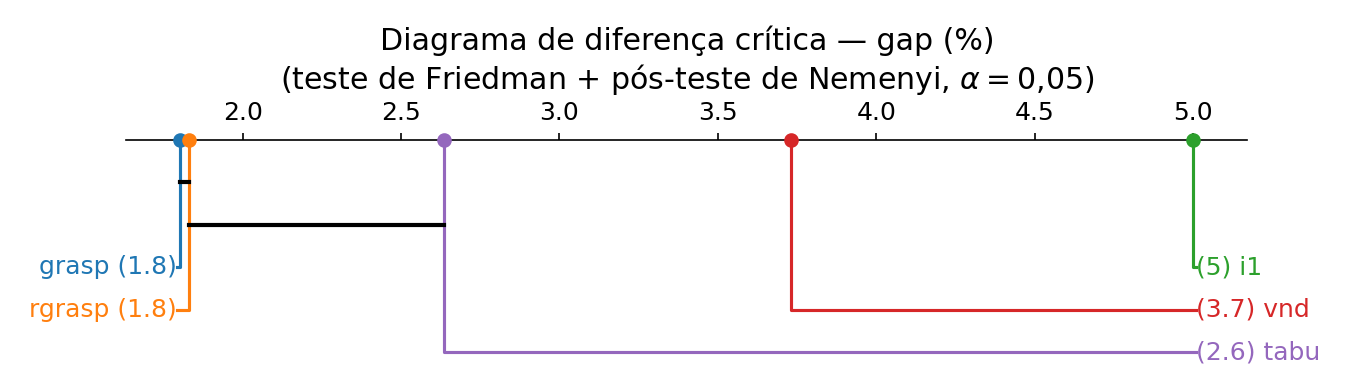
\includegraphics[width=0.85\textwidth]{../../results/figures/cd_diagram_full}
\caption{Diagrama de diferença crítica (Friedman/Nemenyi, 56 instâncias). Cada método aparece na posição do seu rank médio (esquerda = melhor); uma barra horizontal une métodos cuja diferença de ranks é menor que a diferença crítica $CD$ --- estatisticamente indistinguíveis a $5\%$. A leitura correta é dupla: a barra diz quem \emph{não} se separa; a ausência de barra entre dois métodos diz que a diferença observada dificilmente é acaso.}\label{fig:cd}
\end{figure}

\paragraph{Convergência e tempo-alvo (TTT).} A Figura~\ref{fig:conv} mostra a queda do custo ao longo do tempo na instância R101 --- cada curva é o melhor valor corrente de um método, e o formato ``escada'' reflete que o incumbente só muda quando uma solução melhor é encontrada. A análise tempo-alvo (Figura~\ref{fig:ttt}) fixa um alvo de qualidade ($1\%$ acima do melhor conhecido) e pergunta: \emph{quanto tempo o método leva para alcançá-lo?} Cada execução independente fornece um tempo; o gráfico é a distribuição acumulada empírica desses tempos --- curvas mais à esquerda indicam método mais rápido, e a inclinação indica a variabilidade entre execuções. Em R101, $100\%$ das $100$ execuções do GRASP atingiram o alvo.

\begin{figure}[H]
\centering
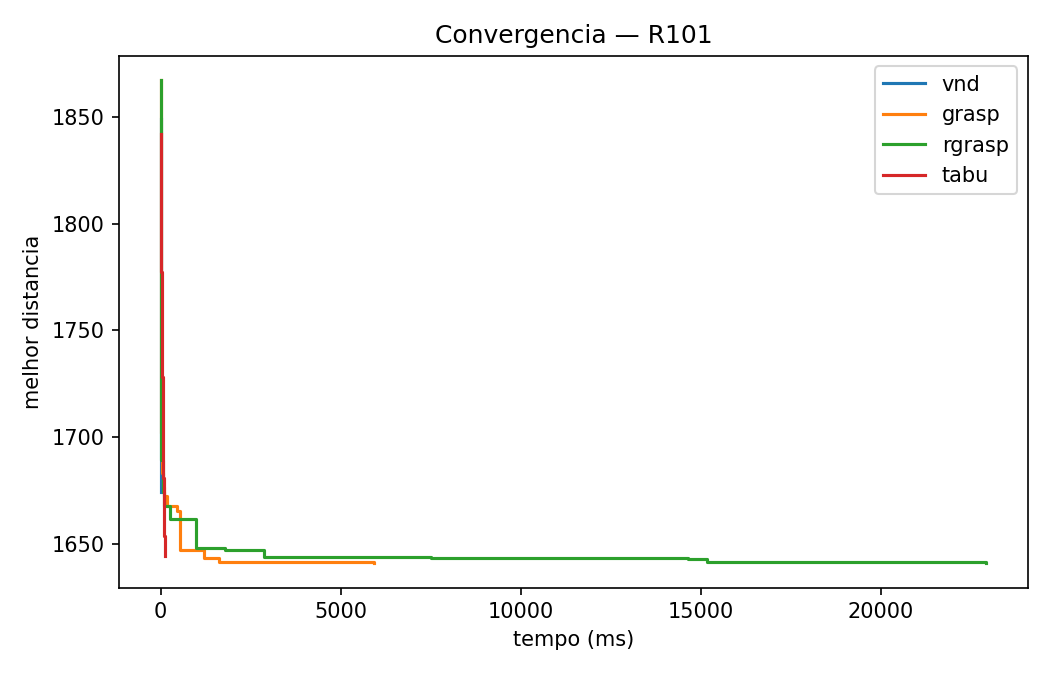
\includegraphics[width=0.7\textwidth]{../../results/figures/convergence_R101}
\caption{Convergência do custo (distância) ao longo do tempo na instância R101.}\label{fig:conv}
\end{figure}

\begin{figure}[H]
\centering
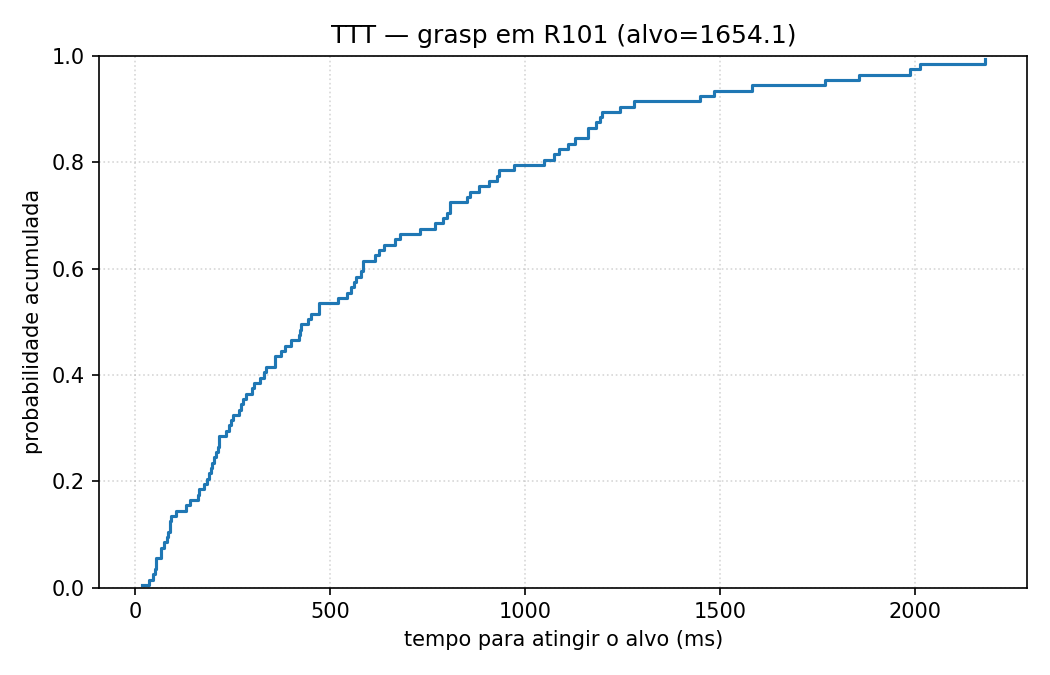
\includegraphics[width=0.7\textwidth]{../../results/figures/ttt_grasp_R101}
\caption{Tempo-alvo (TTT) do GRASP em R101: probabilidade acumulada de atingir o alvo (1\% do melhor conhecido) em função do tempo; 100 execuções.}\label{fig:ttt}
\end{figure}

\subsection{Análise complementar: integral primal (DIMACS)}\label{sec:pi}
A comparação primária deste estudo usa parada por iterações sem melhoria (Seção~\ref{sec:parada}), por reprodutibilidade. Como \emph{complemento}, avaliamos a dimensão \emph{anytime} (tempo $\times$ qualidade) pela métrica oficial da \emph{competição} DIMACS, o \textbf{integral primal} \citep{berthold2013measuring,dimacs12vrptw}: para um orçamento de tempo $T$ e o melhor conhecido $\mathit{BKS}$,
\[
\mathit{PI}=100\left(\frac{\sum_{i} v(i{-}1)\,(t_i-t_{i-1}) + v(n)\,(T-t_n)}{T\cdot \mathit{BKS}} - 1\right),
\]
onde $v(0)=1{,}1\,\mathit{BKS}$ em $t_0=0$ (convenção do desafio: antes da primeira solução, o método é tratado como se estivesse a $10\%$ do melhor conhecido, limitando a penalidade inicial) e $v(i)$ é o valor da incumbente encontrada em $t_i$; menor $\mathit{PI}$ é melhor (encontra boas soluções mais cedo). Reexecutamos os métodos com orçamento de tempo \emph{fixo} ($T=20$\,s) e os parâmetros de qualidade calibrados. \textbf{Ressalva importante:} por depender do tempo de relógio, o integral primal é \emph{dependente da máquina}; por isso é reportado \emph{apenas como complemento} ao estudo reprodutível, e não substitui a comparação primária por iterações.

A Figura~\ref{fig:pi} resume o integral primal médio e a Figura~\ref{fig:anytime} mostra a convergência anytime em R101. % gerado por results_tables.py a partir de primal_integral.csv -- nao editar
O integral primal médio ordena os métodos assim: GRASP ($\mathit{PI}=3{,}08$), GRASP reativo ($\mathit{PI}=3{,}10$), Busca Tabu ($\mathit{PI}=4{,}25$), VND ($\mathit{PI}=8{,}61$) (menor é melhor).
 O VND, embora convirja quase instantaneamente, estaciona em seu ótimo local, o que penaliza seu integral primal; os métodos que continuam melhorando ao longo do tempo obtêm os menores valores. Sob tempo igual a leitura é a mesma da comparação primária, com as distâncias entre os métodos encurtadas --- coerente com o fato de a Busca Tabu realizar muito mais iterações por segundo.

\begin{figure}[H]
\centering
\begin{subfigure}[t]{0.48\textwidth}
\centering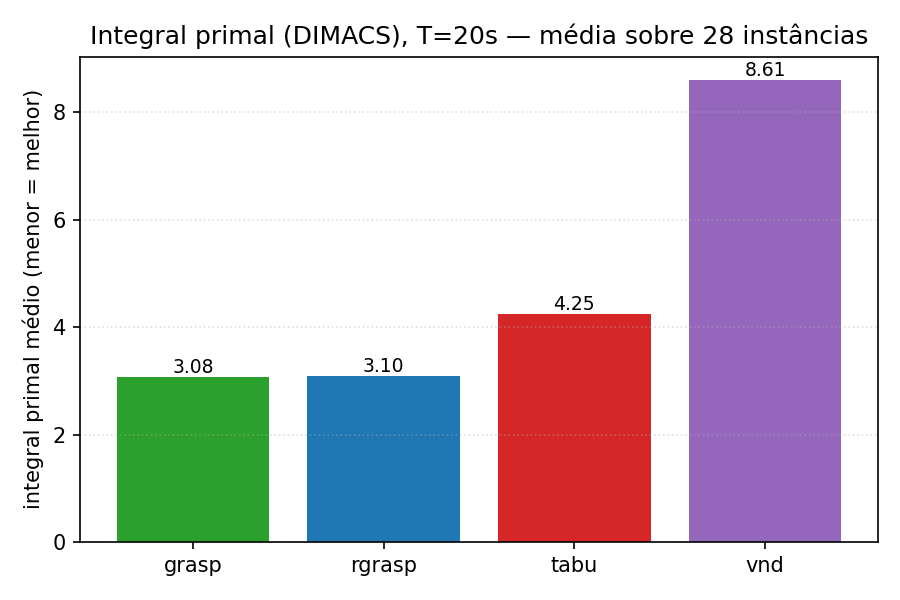
\includegraphics[width=\linewidth]{../../results/figures/primal_integral}
\caption{Integral primal médio (menor = melhor).}\label{fig:pi}
\end{subfigure}\hfill
\begin{subfigure}[t]{0.48\textwidth}
\centering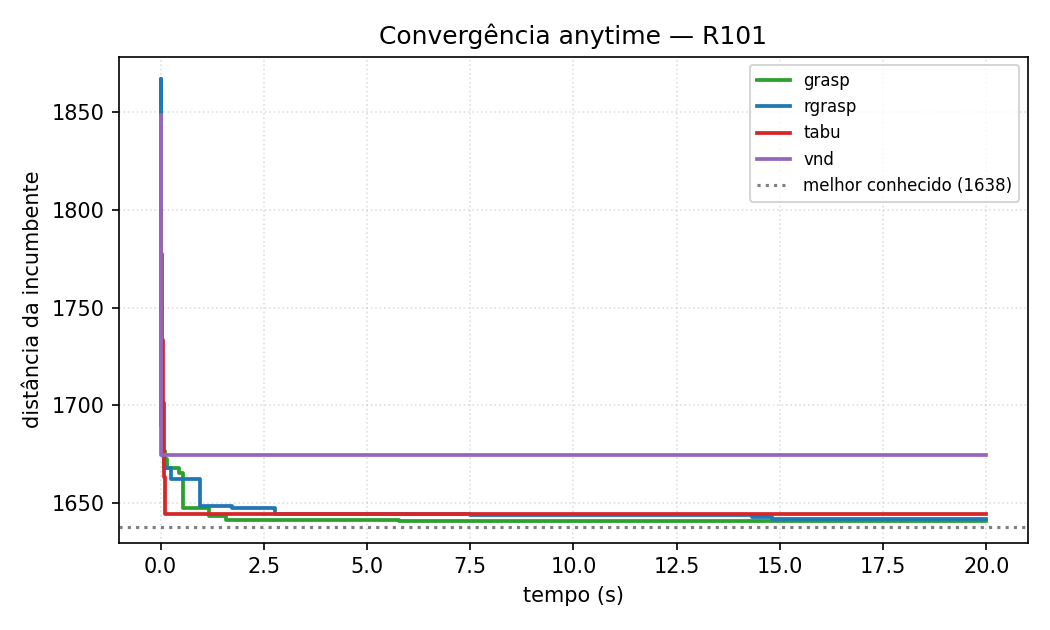
\includegraphics[width=\linewidth]{../../results/figures/anytime_convergence_R101}
\caption{Convergência anytime em R101.}\label{fig:anytime}
\end{subfigure}
\caption{Análise complementar anytime (integral primal do DIMACS, $T=20$\,s). Métrica dependente de máquina, reportada apenas como complemento.}
\end{figure}

\subsection{O baseline e a contagem de veículos}\label{sec:baseline}
O \emph{gap} é medido contra um conjunto de soluções de referência de \textbf{mínima distância} (convenção DIMACS), coerente com o objetivo otimizado, e disponíveis no repositório CVRPLIB \citep{cvrplib} --- repositório oficial do desafio. Coexistem na literatura \emph{três} convenções de arredondamento incompatíveis: a do DIMACS (truncamento a 1 casa decimal, adotada aqui), a do SINTEF (precisão dupla, 2 casas) e a euclidiana real (sem arredondamento); por isso, todos os custos --- nossos e das referências --- são (re)computados sob a \emph{mesma} convenção DIMACS, garantindo comparabilidade. Verificamos que essas referências têm distância menor ou igual à das soluções de \emph{mínimo número de veículos} do repositório SINTEF em todas as 56 instâncias (em 37 estritamente menor; nas demais, iguais), ao custo de utilizarem \emph{mais} veículos. Por exemplo, em R201 a referência de distância usa $8$ veículos com custo $1143{,}2$, enquanto a de mínimo de veículos usa $4$ veículos com custo $1248{,}4$. Portanto, comparar a distância de nossas soluções com esse baseline é coerente, e a contagem ``elevada'' de veículos é a assinatura esperada da minimização de distância --- não um defeito. A Tabela~\ref{tab:lex} reporta a visão lexicográfica (veículos e distância) por família, frente às duas referências. A Tabela~\ref{tab:lex} mostra que nossas soluções superam o SINTEF em distância média usando mais veículos, e aproximam-se da referência de mínima distância; coerentemente, nosso número médio de veículos situa-se entre o das duas referências.

\begin{table}[H]
\centering
\caption{Visão lexicográfica por família: veículos e distância médios das nossas soluções (GRASP, melhor de 30 execuções) e das duas referências --- a de mínima distância (Dinamics/DIMACS) e a de mínimo número de veículos (SINTEF).}\label{tab:lex}
\begin{tabular}{lcccccc}
\toprule
& \multicolumn{2}{c}{\textbf{Nosso (GRASP)}} & \multicolumn{2}{c}{\textbf{Dinamics (mín.\ dist.)}} & \multicolumn{2}{c}{\textbf{SINTEF (mín.\ veíc.)}} \\
\cmidrule(lr){2-3}\cmidrule(lr){4-5}\cmidrule(lr){6-7}
\textbf{Família} & veíc. & dist. & veíc. & dist. & veíc. & dist. \\
\midrule
C (agrupada) & 6{,}7 & 714{,}3 & 6{,}7 & 714{,}1 & 6{,}7 & 714{,}1 \\
R (aleatória) & 9{,}0 & 1042{,}7 & 9{,}5 & 1029{,}6 & 7{,}5 & 1081{,}9 \\
RC (mista) & 9{,}1 & 1184{,}2 & 9{,}4 & 1167{,}6 & 7{,}4 & 1248{,}3 \\
\midrule
Todas & 8{,}3 & 983{,}4 & 8{,}6 & 973{,}2 & 7{,}2 & 1017{,}8 \\
\bottomrule
\end{tabular}
\end{table}


% ============================================================
\section{Aplicação: Digital Twin para coleta de resíduos}\label{sec:twin}

Como terceira camada, um \textit{Digital Twin} transfere os algoritmos \emph{calibrados no benchmark} para um cenário de coleta de resíduos. Trata-se de uma \textbf{prova de conceito}: as localizações são reais, mas o comportamento de enchimento é simulado.

\paragraph{Dados e enquadramento.} Usamos as localizações reais de \textbf{38 pontos de entrega voluntária (PEVs)} de coleta seletiva de Vitória/ES, obtidas do serviço de dados abertos do município, com o depósito na associação de triagem AMARIV. O \emph{nível de enchimento} de cada lixeira é gerado por um \textbf{processo de Poisson não-homogêneo} (NHPP) discretizado em ciclos ($8$ ciclos/dia $\approx 3$\,h cada). Em cada ciclo $c$, a intensidade é
\begin{equation}
\lambda(c)=\lambda_{\mathrm{off}}+(\lambda_{\mathrm{pico}}-\lambda_{\mathrm{off}})\,\min\!\big(1,\,\rho(c)\big),\qquad
\rho(c)=e^{-(h-1{,}5)^2}+e^{-(h-5{,}5)^2},\quad h=c\bmod 8,
\end{equation}
com $\lambda_{\mathrm{off}}=0{,}8$ e $\lambda_{\mathrm{pico}}=4{,}0$ (dois picos diários). O número de chegadas na lixeira $i$ no ciclo é $\mathrm{Poisson}\big(\lambda(c)\,p_i\big)$, com propensão heterogênea $p_i\sim\mathcal{U}(0{,}5;\,1{,}5)$, e o enchimento sobe $\Delta f=\text{chegadas}/12$. Uma lixeira transborda se $f$ atinge $1$ antes de ser coletada (KPI rastreado). Registre-se que \emph{o enchimento é sintético}, calibrado pela literatura de resíduos urbanos \citep{lozano2018smart,barth2023data}, pois a coleta de séries reais exigiria meses de monitoramento --- fora do escopo de uma Iniciação Científica. A validação com dados reais de enchimento é trabalho futuro.

\subsection{Camada de comunicação LoRaWAN (simulada)}\label{sec:lorawan}
Entre os sensores e o orquestrador há uma camada de comunicação que simula os efeitos relevantes de uma rede LoRaWAN na escala de um ciclo de monitoramento. Sensores de lixeira alimentados por bateria operam tipicamente na classe A do LoRaWAN --- o dispositivo passa a maior parte do tempo dormindo e acorda apenas para transmitir --- com \emph{uplinks} não confirmados (sem retransmissão); três efeitos dessa escolha são modelados. A \textbf{perda de pacote}: cada uplink é entregue com probabilidade $\mathit{pdr}$ (\emph{packet delivery ratio}, padrão $0{,}98$), e um pacote perdido não é retransmitido. O \textbf{ciclo de \textit{duty}}: a banda ISM limita o tempo de ar de cada dispositivo (cerca de $1\%$ na faixa EU868), o que na prática limita a frequência de transmissão --- cada sensor transmite a cada $\mathit{duty}$ ciclos, com fases sorteadas para que a rede não transmita em uníssono. A \textbf{defasagem}: o atraso fim-a-fim de um uplink (segundos) é desprezível frente a um ciclo (horas), de modo que o efeito real da latência nessa escala é a \emph{idade} da leitura --- entre transmissões, ou após uma perda, o orquestrador segue operando com a última leitura recebida.

A consequência é uma distinção que o gêmeo digital passa a representar: o roteador não decide sobre o estado físico das lixeiras, e sim sobre a \emph{visão de rádio} desse estado. O acionamento por limiar, a demanda e a janela dinâmica usam o valor percebido; o transbordo continua contado no estado físico, que é o que ocorre na rua. Uma lixeira que cruza o limiar mas perde o uplink fica invisível ao planejamento até o próximo uplink entregue, e o transbordo que ocorrer nesse intervalo é atribuível à comunicação --- um custo operacional que o modelo sem camada de rádio não capturava. Com canal perfeito ($\mathit{pdr}=1$, transmissão a cada ciclo) a camada é transparente e o comportamento reproduz exatamente o do gêmeo sem ela, propriedade verificada por comparação direta das duas execuções. O efeito do canal é mensurável: no mapa R101 com 12 ciclos e o VND como roteador, degradar o canal para $\mathit{pdr}=0{,}9$ com transmissão a cada 2 ciclos elevou os transbordos de $35$ para $104$, com defasagem média de $0{,}52$ ciclo --- a qualidade da comunicação, e não apenas a do roteamento, limita o serviço.

\subsection{Malha viária real (distâncias e tempos de direção)}\label{sec:road}
Para realismo, além do grafo euclidiano (linha reta entre pontos), construímos um \textbf{grafo viário real}: a matriz de \emph{distância} (metros) e a matriz de \emph{tempo} (segundos de direção) entre o depósito e os 38 PEVs são obtidas da malha do OpenStreetMap pelo serviço de roteamento OSRM, e a geometria de $5\,937$ ruas é usada para visualização. O fator de circuito médio (distância rodoviária / linha reta) foi de \textbf{1{,}53} (até $6{,}9$ em pares separados por água, já que Vitória é uma ilha). O solver foi estendido para aceitar matrizes \emph{explícitas} de distância e tempo (o \textit{benchmark} euclidiano de Solomon permanece inalterado, pois suas execuções não usam matrizes): assim o custo otimizado passa a ser a distância \emph{rodoviária} e as janelas/espera usam o tempo \emph{real} de direção. O cenário rodoviário é internamente consistente em \emph{unidades físicas} --- distância em metros, e tempo, janelas e serviço em segundos ($H=6$\,h, serviço $=120$\,s) ---, independentes das unidades abstratas do \textit{benchmark}. A Figura~\ref{fig:road} mostra as rotas resultantes seguindo as ruas reais; rotear os 38 PEVs produziu 6 veículos, $83{,}6$\,km de percurso viário e $3{,}7$\,h de operação.

\begin{figure}[H]
\centering
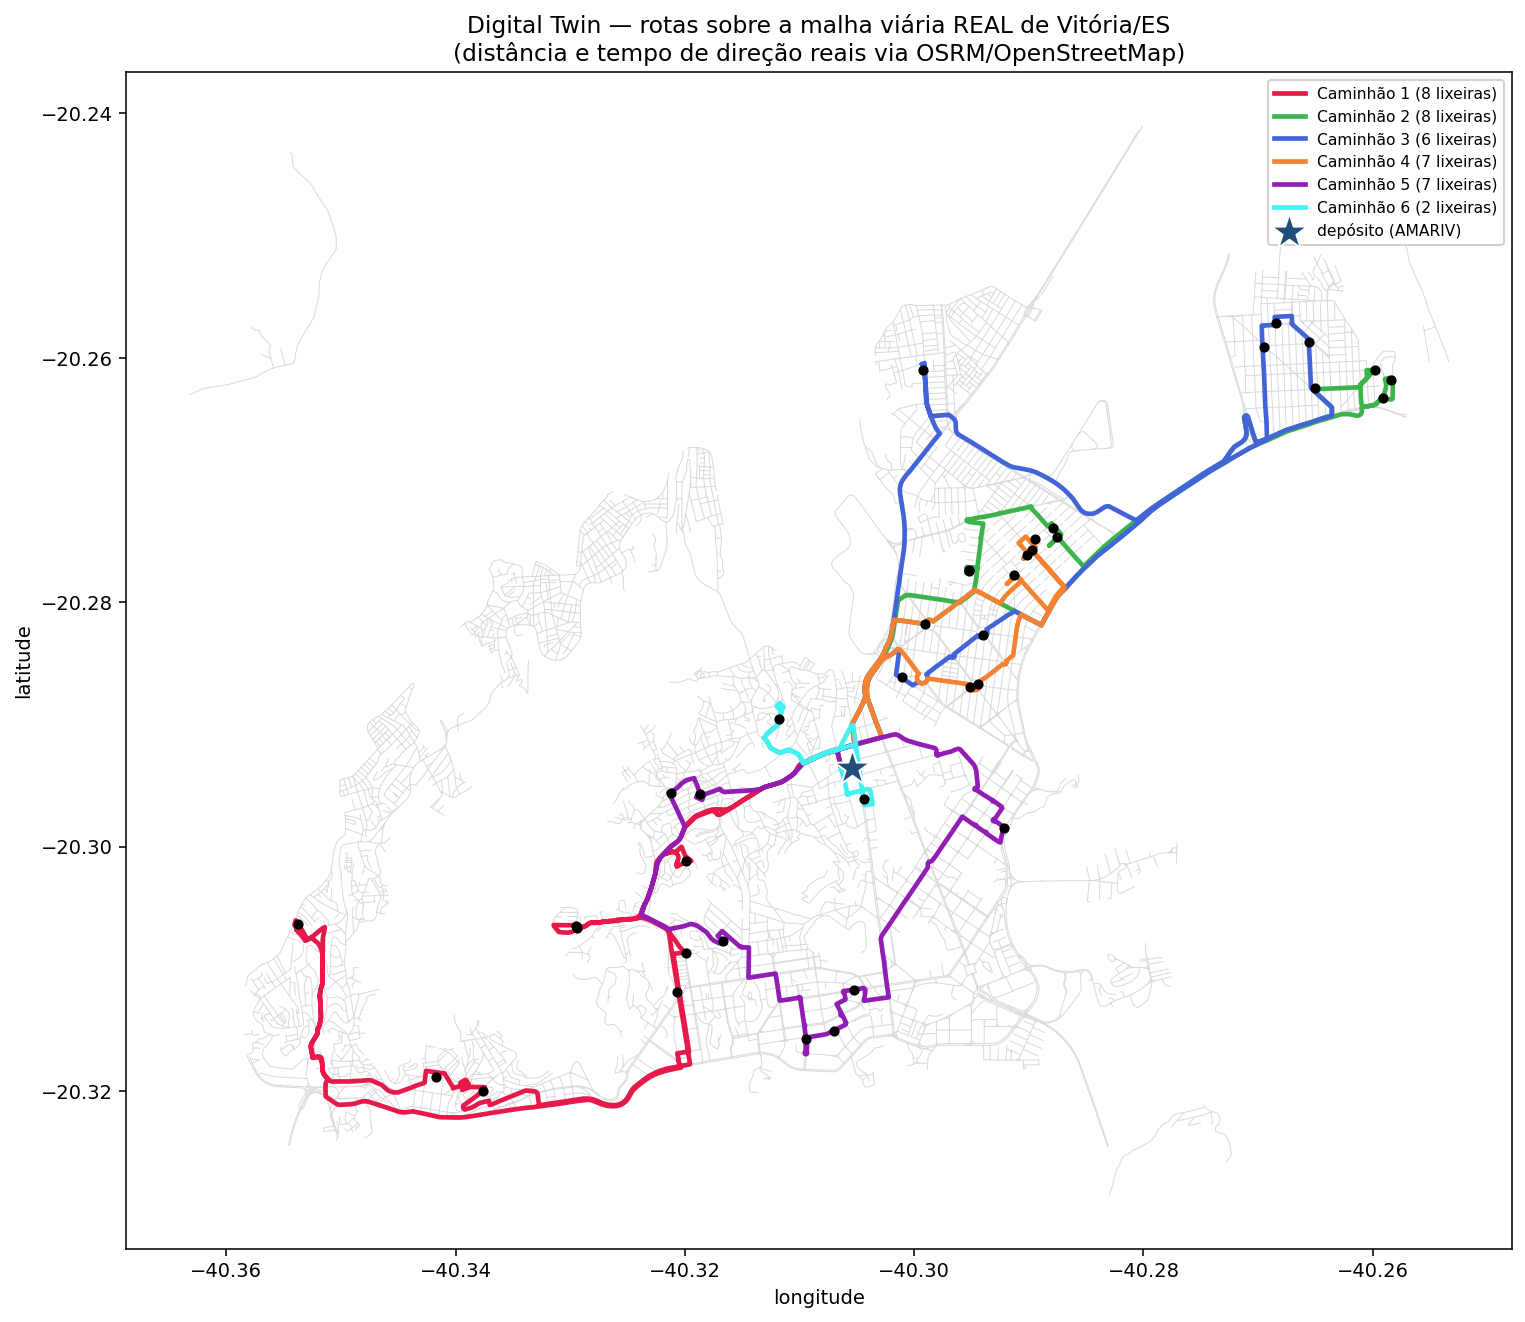
\includegraphics[width=0.82\textwidth]{../../results/digital_twin/vitoria/vitoria_road_routes}
\caption{Rotas do Digital Twin sobre a malha viária \emph{real} de Vitória/ES (OSM): cada cor é um caminhão, traçado pela geometria de direção real (OSRM); a estrela é o depósito (AMARIV).}\label{fig:road}
\end{figure}

\subsection{Modelo do cenário: capacidades, tempo e espera}\label{sec:modelo}
Para que não haja qualquer ambiguidade, definimos formalmente cada elemento do cenário de coleta.

\textbf{Capacidade do veículo ($Q$).} Cada caminhão carrega no máximo $Q$ unidades de demanda. Ao longo de uma rota, a carga acumulada é a soma das demandas das lixeiras visitadas; \emph{nenhuma} rota pode exceder $Q$. Quando incluir mais uma lixeira excederia $Q$, a rota é fechada (o caminhão retorna ao depósito) e outro veículo é necessário --- é isto que, junto com as janelas, determina o \emph{número de veículos}.

\textbf{Capacidade da lixeira e demanda.} O estado de cada lixeira é o nível de enchimento $f\in[0,1]$ ($0$ = vazia, $1$ = cheia/transbordando). O enchimento sobe pelo processo de Poisson não-homogêneo; ao atingir $1$, a lixeira \emph{transborda} (indicador de falha de serviço). A demanda de coleta é derivada do enchimento por $\mathrm{demanda}=\operatorname{round}(9f)+1$ (arredondamento ao inteiro mais próximo; entre $1$ e $10$): é uma medida de \emph{prioridade/volume a recolher}, \emph{não} o peso físico --- lixeiras mais cheias recebem demanda maior e ocupam mais da capacidade do veículo.

\textbf{Tempo, chegada e espera.} O tempo de viagem entre dois pontos é a \emph{duração real de direção} pela malha viária (segundos, OSRM); no grafo euclidiano, é proporcional à distância (velocidade constante). Partindo do depósito em $t=0$, a cada perna da rota: $\text{chegada} = \text{partida}_{\text{anterior}} + \text{tempo de viagem}$. Se a chegada ocorre \emph{antes} da abertura da janela da lixeira ($\mathit{ready}$), o veículo \textbf{espera, ocioso}, até $\mathit{ready}$: o início de serviço é $\text{início}=\max(\text{chegada},\mathit{ready})$. O serviço dura $\mathit{service}$ segundos e $\text{partida}=\text{início}+\mathit{service}$. A rota deve retornar ao depósito até o fim do horizonte ($\mathit{due}$ do depósito). Uma janela é \emph{violada} (solução inviável) se $\text{início}>\mathit{due}$ da lixeira. Este é exatamente o mecanismo ilustrado numericamente no exemplo da Seção~\ref{sec:exemplos}(a).

\paragraph{Janelas de tempo dinâmicas.} A cada ciclo de monitoramento, as lixeiras acima de um limiar de enchimento $\tau$ tornam-se demandas de coleta com \textbf{janela de tempo dinâmica} $[\,0,\,\mathit{due}\,]$: quanto mais cheia (mais crítica) a lixeira, mais cedo seu prazo. Formalmente, com criticidade $\mathrm{crit}=\max\!\big(0,\,(f-\tau)/(1-\tau)\big)\in[0,1]$,
\begin{equation}
\mathit{due}=H\,\big(1-\kappa\cdot\mathrm{crit}\big),
\end{equation}
onde $H$ é o horizonte e $\kappa$ (padrão $0{,}6$) é o \emph{coeficiente de urgência} --- analisado na sensibilidade (Figura~\ref{fig:sens}). Isso explora diretamente o critério Push Forward do solver (Seção~\ref{sec:invariantes}), priorizando as lixeiras críticas. Constrói-se então uma instância VRPTW e invoca-se o solver (com os parâmetros calibrados) para (re)planejar as rotas; as lixeiras atendidas são esvaziadas.

\paragraph{O que influencia o número de veículos e o esvaziamento das rotas.} Três fatores governam a operação simulada e explicam o comportamento do sistema: (i) o \emph{limiar de acionamento} --- limiares menores acionam mais lixeiras por ciclo, exigindo mais veículos; (ii) a \emph{capacidade do veículo} frente à \emph{demanda} de cada lixeira (que cresce com o enchimento, como heurística de priorização) --- quanto menor a razão capacidade/demanda, mais rotas; e (iii) as \emph{janelas dinâmicas} --- prazos mais apertados reduzem o compartilhamento de rotas e podem aumentar o número de veículos. Uma rota ``esvazia'' (e um veículo é liberado) quando os movimentos entre rotas conseguem redistribuir todos os seus clientes sem violar viabilidade.

\paragraph{Validação estático vs.\ dinâmico.} Comparam-se dois regimes sobre a \emph{mesma} realização de enchimento: o \textbf{dinâmico} (coleta sob demanda das lixeiras acima do limiar a cada ciclo) e o \textbf{estático} (coleta de todas as lixeiras a cada $f$ ciclos, independentemente do enchimento). Os indicadores são distância total, número de coletas e \textbf{transbordos}. Como os parâmetros operacionais (limiar, capacidade, frequência $f$, coeficiente de urgência) são escolhas de modelagem, reportamos uma \textbf{análise de sensibilidade} variando-os, em vez de fixá-los arbitrariamente; e não estendemos as conclusões além do que a simulação suporta. Um painel interativo (\textit{dashboard}) permite reproduzir e visualizar os ciclos.

\paragraph{Resultados (prova de conceito em Vitória/ES).} Sobre uma simulação de 16 ciclos com a mesma realização de enchimento e o canal LoRaWAN padrão ($\mathit{pdr}=0{,}98$), o regime \textbf{dinâmico} alcançou distância ligeiramente menor que o \textbf{estático} com \emph{metade das coletas} e \emph{menos transbordos} (Tabela~\ref{tab:twin}) --- coletar sob demanda, guiado pelos sensores, atende melhor com menos esforço. Parte dos transbordos do regime dinâmico é atribuível à comunicação, não ao roteamento: com o canal degradado da Seção~\ref{sec:lorawan}, essa parcela cresce. Aplicando os cinco algoritmos à mesma simulação, os métodos de melhoria convergem a rotas de custo muito próximo: nas instâncias \emph{pequenas} de cada ciclo (tipicamente 10--20 lixeiras ativas), a diferença entre as meta-heurísticas quase desaparece --- as distinções medidas no \textit{benchmark} de 100 clientes manifestam-se em problemas maiores.

\begin{table}[H]
\centering
\caption{Gêmeo digital (Vitória/ES, 16 ciclos, mesma realização de enchimento e canal LoRaWAN com $\mathit{pdr}=0{,}98$): coleta dinâmica guiada pelos sensores contra coleta estática de frequência fixa (a cada 3 ciclos). O regime estático não usa sensores --- coleta todas as lixeiras no dia programado.}\label{tab:twin}
\begin{tabular}{lcccc}
\toprule
\textbf{Regime} & \textbf{Distância} & \textbf{Coletas} & \textbf{Transbordos} & \textbf{Ciclos com rota} \\
\midrule
Dinâmico (sob demanda) & 3516{,}9 & 117 & \textbf{21} & 15 \\
Estático (a cada 3 ciclos) & 3562{,}1 & 228 & 25 & 6 \\
\bottomrule
\end{tabular}
\end{table}


\paragraph{Sensibilidade dos parâmetros.} Como os parâmetros do cenário são escolhas de modelagem, analisamos sua sensibilidade (Figura~\ref{fig:sens}) em vez de fixá-los arbitrariamente. O \emph{limiar de coleta} domina o compromisso serviço--custo: limiares mais altos reduzem coletas mas aumentam transbordos (de $2$ a $40$ ao variar de $50\%$ a $90\%$). A \emph{capacidade} do veículo reduz fortemente a distância (de $6667$ a $3097$ ao variar de $15$ a $40$), sem afetar transbordos. O \emph{coeficiente de urgência}, por sua vez, tem efeito agregado pequeno nos indicadores: ele atua sobretudo na \emph{priorização} (ordem de atendimento) dentro de rotas que permanecem viáveis. Esses resultados justificam a escolha dos valores padrão e delimitam o papel de cada parâmetro.

\begin{figure}[H]
\centering
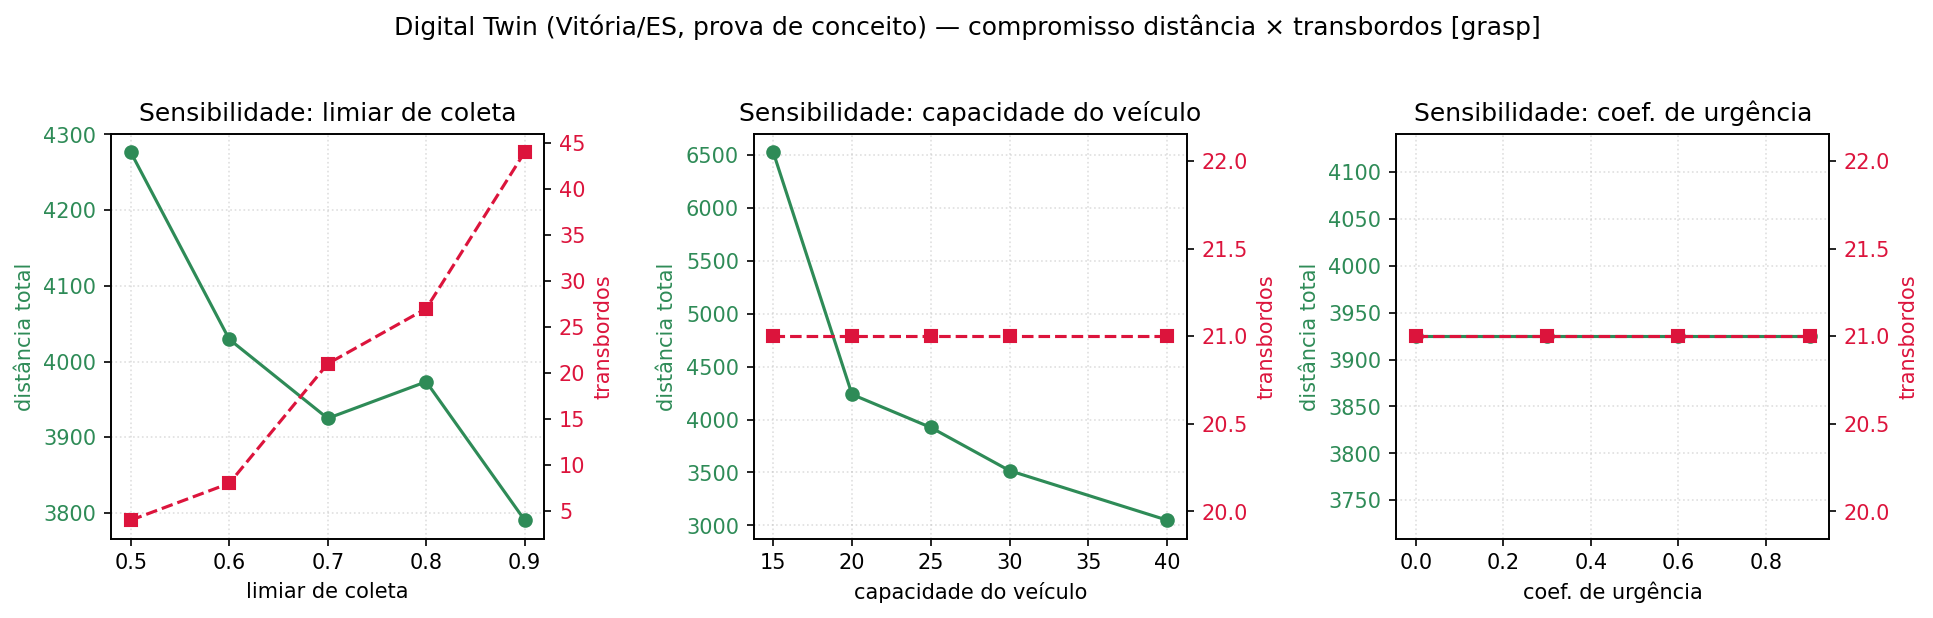
\includegraphics[width=\textwidth]{../../results/digital_twin/sensitivity}
\caption{Análise de sensibilidade do Digital Twin: compromisso distância (verde) $\times$ transbordos (vermelho) ao variar limiar, capacidade e coeficiente de urgência.}\label{fig:sens}
\end{figure}

% ============================================================
\section{Atividades realizadas}\label{sec:atividades}
As Etapas~1 a~3 (revisão bibliográfica, aprofundamento no algoritmo de Solomon e nas tecnologias de sensores, e definição da arquitetura) foram concluídas. A Etapa~4 (implementação dos algoritmos e do ambiente de simulação) foi concluída: o solver com os cinco métodos sobre o núcleo compartilhado está implementado, testado e verificado. A Etapa~5 (relatório parcial) foi entregue. As Etapas~6 e~7 (Digital Twin e testes computacionais) encontram-se avançadas: a calibração por \textit{irace}, a comparação estatística nas 56 instâncias e o Digital Twin com dados reais de Vitória já estão operacionais. As Etapas~8 e~9 (análise final e relatório) estão em finalização com este documento. Em relação ao relatório parcial, houve avanço de cronograma: as atividades antes previstas como futuras (6--7) já produzem resultados.

% ============================================================
\section{Conclusão}\label{sec:conclusao}
Este trabalho estabeleceu uma comparação \emph{justa, reprodutível e verificável} de cinco heurísticas clássicas para o VRPTW, sobre um núcleo compartilhado, com viabilidade garantida por construção e por verificação independente, parada por iterações sem melhoria (reprodutível) e comparação estatística por Friedman/Nemenyi. As escolhas metodológicas --- objetivo, baseline, conjunto de vizinhanças e calibração --- foram justificadas explicitamente, inclusive empiricamente (ablação) e por verificação contra referências publicadas.

Quantitativamente, a hierarquia empírica é $\{\text{GRASP} \approx \text{GRASP reativo}\} \succ \text{Busca Tabu} \succ \text{VND} \succ \text{I1}$: cada camada de refinamento reduz o gap médio de distância --- de $35{,}97\%$ (construção I1 pura) para $8{,}43\%$ (VND) e para menos de $2\%$ nas duas variantes de GRASP, com a Busca Tabu em posição intermediária ($3{,}95\%$) --- e todas as separações são estatisticamente significativas no conjunto de teste (Wilcoxon com Holm), exceto entre o GRASP fixo e o reativo, indistinguíveis. Sobre a calibração, o resultado é diferenciado e honesto: ela rendeu ganho demonstrável para a Busca Tabu ($+1{,}26$~pp), foi marginal para o Reativo e não superou o valor clássico da literatura para o GRASP --- que se mostrou insensível a $\alpha$ na faixa estudada e, pelo protocolo pré-declarado, usa o valor clássico no estudo final. A verificação reproduziu os $56$ custos de referência e \emph{nenhuma} das $3\,528$ execuções do estudo produziu solução inviável, confirmando que os algoritmos de melhoria respeitam cobertura, capacidade e janelas de tempo a cada passo. Transportados ao Digital Twin de coleta em Vitória/ES --- agora incluindo a camada de comunicação LoRaWAN simulada ---, os algoritmos mostraram que a coleta dinâmica guiada por sensores atende com metade das coletas e menos transbordos que a coleta de frequência fixa, e que a qualidade do canal de comunicação, não apenas a do roteamento, limita o serviço.

\paragraph{Limitações.} O objetivo otimizado é a distância (DIMACS); a abordagem lexicográfica de Solomon foi reportada apenas de forma complementar. A Busca Tabu foi mantida na forma mais simples (sem diversificação avançada). No Digital Twin, o enchimento das lixeiras é simulado, não medido; a comunicação LoRaWAN é representada, não validada energeticamente.

\paragraph{Trabalhos futuros.} Validação com dados reais de enchimento em Vitória (piloto com sensores); avaliação sob o critério lexicográfico veículos$\rightarrow$distância; variantes mais ricas (Tabu com memória de longo prazo, metaheurísticas híbridas/ILS); e quantificação de benefícios econômicos e ambientais.

% ============================================================
\appendix
\section{Resultados detalhados por instância}\label{ap:porinstancia}
A Tabela~\ref{tab:porinstancia} apresenta, para cada uma das 56 instâncias, a comparação dos cinco algoritmos nas métricas: número de veículos, custo (distância média), gap percentual ao melhor conhecido, número de iterações e tempo. Para os algoritmos estocásticos (GRASP e GRASP reativo), iterações e tempo são médias sobre as 30 execuções. O menor gap de cada instância é destacado em negrito.

% Gerado por experiments/analysis/per_instance_table.py — NÃO editar à mão.
{\footnotesize
\begin{longtable}{llrrrrr}
\caption{Resultados por instância: comparação dos cinco algoritmos. Custo = distância média; Gap em \% ao melhor conhecido; Iter.\ e Tempo são médias (30 execuções para os estocásticos). O menor gap de cada instância está em negrito.}\label{tab:porinstancia}\\
\toprule
\textbf{Instância} & \textbf{Alg.} & \textbf{Veíc.} & \textbf{Custo} & \textbf{Gap (\%)} & \textbf{Iter.} & \textbf{Tempo (s)} \\
\midrule
\endfirsthead
\multicolumn{7}{l}{\footnotesize\itshape continuação da Tabela~\ref{tab:porinstancia}}\\
\toprule
\textbf{Instância} & \textbf{Alg.} & \textbf{Veíc.} & \textbf{Custo} & \textbf{Gap (\%)} & \textbf{Iter.} & \textbf{Tempo (s)} \\
\midrule
\endhead
\midrule \multicolumn{7}{r}{\footnotesize\itshape continua na próxima página}\\
\endfoot
\bottomrule
\endlastfoot
\multirow{5}{*}{C101}
  & I1 & 10,0 & 922,0 & 11,45 & 0 & 0,00 \\
  & \textbf{VND} & 10,0 & 827,3 & \textbf{0,00} & 0 & 0,01 \\
  & \textbf{GRASP} & 10,0 & 827,3 & \textbf{0,00} & 802 & 15,74 \\
  & \textbf{GRASP-R} & 10,0 & 827,3 & \textbf{0,00} & 801 & 15,19 \\
  & \textbf{Tabu} & 10,0 & 827,3 & \textbf{0,00} & 806 & 8,64 \\
\midrule
\multirow{5}{*}{C102}
  & I1 & 10,0 & 1039,7 & 25,67 & 0 & 0,00 \\
  & \textbf{VND} & 10,0 & 827,3 & \textbf{0,00} & 0 & 0,02 \\
  & \textbf{GRASP} & 10,0 & 827,3 & \textbf{0,00} & 806 & 32,66 \\
  & \textbf{GRASP-R} & 10,0 & 827,3 & \textbf{0,00} & 801 & 28,76 \\
  & \textbf{Tabu} & 10,0 & 827,3 & \textbf{0,00} & 816 & 4,90 \\
\midrule
\multirow{5}{*}{C103}
  & I1 & 11,0 & 1221,7 & 47,85 & 0 & 0,00 \\
  & VND & 10,0 & 881,0 & 6,62 & 0 & 0,03 \\
  & \textbf{GRASP} & 10,0 & 826,3 & \textbf{0,00} & 870 & 40,96 \\
  & \textbf{GRASP-R} & 10,0 & 826,3 & \textbf{0,00} & 811 & 34,90 \\
  & \textbf{Tabu} & 10,0 & 826,3 & \textbf{0,00} & 1027 & 5,52 \\
\midrule
\multirow{5}{*}{C104}
  & I1 & 10,0 & 1148,2 & 39,53 & 0 & 0,00 \\
  & VND & 10,0 & 876,7 & 6,54 & 0 & 0,02 \\
  & GRASP & 10,0 & 825,2 & 0,29 & 1518 & 65,56 \\
  & \textbf{GRASP-R} & 10,0 & 822,9 & \textbf{0,00} & 857 & 32,84 \\
  & \textbf{Tabu} & 10,0 & 822,9 & \textbf{0,00} & 1662 & 9,54 \\
\midrule
\multirow{5}{*}{C105}
  & I1 & 10,0 & 878,9 & 6,24 & 0 & 0,00 \\
  & \textbf{VND} & 10,0 & 827,3 & \textbf{0,00} & 0 & 0,01 \\
  & \textbf{GRASP} & 10,0 & 827,3 & \textbf{0,00} & 803 & 20,51 \\
  & \textbf{GRASP-R} & 10,0 & 827,3 & \textbf{0,00} & 801 & 17,85 \\
  & \textbf{Tabu} & 10,0 & 827,3 & \textbf{0,00} & 806 & 8,65 \\
\midrule
\multirow{5}{*}{C106}
  & I1 & 11,0 & 951,2 & 14,98 & 0 & 0,00 \\
  & \textbf{VND} & 10,0 & 827,3 & \textbf{0,00} & 0 & 0,01 \\
  & \textbf{GRASP} & 10,0 & 827,3 & \textbf{0,00} & 803 & 23,95 \\
  & \textbf{GRASP-R} & 10,0 & 827,3 & \textbf{0,00} & 801 & 20,35 \\
  & \textbf{Tabu} & 10,0 & 827,3 & \textbf{0,00} & 812 & 4,33 \\
\midrule
\multirow{5}{*}{C107}
  & I1 & 10,0 & 902,4 & 9,08 & 0 & 0,00 \\
  & \textbf{VND} & 10,0 & 827,3 & \textbf{0,00} & 0 & 0,01 \\
  & \textbf{GRASP} & 10,0 & 827,3 & \textbf{0,00} & 805 & 25,12 \\
  & \textbf{GRASP-R} & 10,0 & 827,3 & \textbf{0,00} & 801 & 19,90 \\
  & \textbf{Tabu} & 10,0 & 827,3 & \textbf{0,00} & 806 & 8,25 \\
\midrule
\multirow{5}{*}{C108}
  & I1 & 10,0 & 975,2 & 17,88 & 0 & 0,00 \\
  & \textbf{VND} & 10,0 & 827,3 & \textbf{0,00} & 0 & 0,01 \\
  & \textbf{GRASP} & 10,0 & 827,3 & \textbf{0,00} & 812 & 27,47 \\
  & \textbf{GRASP-R} & 10,0 & 827,3 & \textbf{0,00} & 802 & 22,70 \\
  & \textbf{Tabu} & 10,0 & 827,3 & \textbf{0,00} & 819 & 4,37 \\
\midrule
\multirow{5}{*}{C109}
  & I1 & 11,0 & 933,1 & 12,79 & 0 & 0,00 \\
  & VND & 10,0 & 847,5 & 2,44 & 0 & 0,01 \\
  & \textbf{GRASP} & 10,0 & 827,3 & \textbf{0,00} & 822 & 28,07 \\
  & \textbf{GRASP-R} & 10,0 & 827,3 & \textbf{0,00} & 803 & 23,85 \\
  & \textbf{Tabu} & 10,0 & 827,3 & \textbf{0,00} & 821 & 4,79 \\
\midrule
\multirow{5}{*}{C201}
  & I1 & 3,0 & 609,1 & 3,40 & 0 & 0,00 \\
  & \textbf{VND} & 3,0 & 589,1 & \textbf{0,00} & 0 & 0,01 \\
  & \textbf{GRASP} & 3,0 & 589,1 & \textbf{0,00} & 801 & 8,24 \\
  & \textbf{GRASP-R} & 3,0 & 589,1 & \textbf{0,00} & 801 & 10,80 \\
  & \textbf{Tabu} & 3,0 & 589,1 & \textbf{0,00} & 801 & 14,42 \\
\midrule
\multirow{5}{*}{C202}
  & I1 & 4,0 & 793,0 & 34,61 & 0 & 0,00 \\
  & VND & 3,0 & 617,9 & 4,89 & 0 & 0,03 \\
  & \textbf{GRASP} & 3,0 & 589,1 & \textbf{0,00} & 802 & 32,52 \\
  & \textbf{GRASP-R} & 3,0 & 589,1 & \textbf{0,00} & 802 & 36,21 \\
  & Tabu & 3,0 & 617,9 & 4,89 & 815 & 6,68 \\
\midrule
\multirow{5}{*}{C203}
  & I1 & 4,0 & 931,4 & 58,21 & 0 & 0,00 \\
  & VND & 4,0 & 635,3 & 7,92 & 0 & 0,05 \\
  & GRASP & 3,0 & 592,0 & 0,56 & 1066 & 61,81 \\
  & GRASP-R & 3,0 & 589,0 & 0,05 & 1158 & 71,65 \\
  & \textbf{Tabu} & 3,0 & 588,7 & \textbf{0,00} & 929 & 8,61 \\
\midrule
\multirow{5}{*}{C204}
  & I1 & 4,0 & 1138,4 & 93,57 & 0 & 0,00 \\
  & VND & 4,0 & 689,7 & 17,28 & 0 & 0,08 \\
  & GRASP & 3,0 & 596,9 & 1,50 & 1213 & 83,57 \\
  & \textbf{GRASP-R} & 3,0 & 596,7 & \textbf{1,47} & 1503 & 108,00 \\
  & Tabu & 4,0 & 620,5 & 5,51 & 1220 & 9,62 \\
\midrule
\multirow{5}{*}{C205}
  & I1 & 4,0 & 667,6 & 13,85 & 0 & 0,00 \\
  & VND & 3,0 & 606,8 & 3,48 & 0 & 0,01 \\
  & \textbf{GRASP} & 3,0 & 586,4 & \textbf{0,00} & 802 & 14,88 \\
  & \textbf{GRASP-R} & 3,0 & 586,4 & \textbf{0,00} & 803 & 16,18 \\
  & \textbf{Tabu} & 3,0 & 586,4 & \textbf{0,00} & 812 & 6,70 \\
\midrule
\multirow{5}{*}{C206}
  & I1 & 3,0 & 660,6 & 12,73 & 0 & 0,00 \\
  & \textbf{VND} & 3,0 & 586,0 & \textbf{0,00} & 0 & 0,01 \\
  & \textbf{GRASP} & 3,0 & 586,0 & \textbf{0,00} & 801 & 20,53 \\
  & \textbf{GRASP-R} & 3,0 & 586,0 & \textbf{0,00} & 801 & 20,50 \\
  & \textbf{Tabu} & 3,0 & 586,0 & \textbf{0,00} & 810 & 6,66 \\
\midrule
\multirow{5}{*}{C207}
  & I1 & 3,0 & 747,1 & 27,54 & 0 & 0,00 \\
  & \textbf{VND} & 3,0 & 585,8 & \textbf{0,00} & 0 & 0,02 \\
  & \textbf{GRASP} & 3,0 & 585,8 & \textbf{0,00} & 801 & 19,95 \\
  & \textbf{GRASP-R} & 3,0 & 585,8 & \textbf{0,00} & 801 & 20,60 \\
  & \textbf{Tabu} & 3,0 & 585,8 & \textbf{0,00} & 814 & 6,67 \\
\midrule
\multirow{5}{*}{C208}
  & I1 & 3,0 & 717,6 & 22,50 & 0 & 0,00 \\
  & VND & 3,0 & 632,3 & 7,94 & 0 & 0,02 \\
  & \textbf{GRASP} & 3,0 & 585,8 & \textbf{0,00} & 801 & 23,57 \\
  & \textbf{GRASP-R} & 3,0 & 585,8 & \textbf{0,00} & 801 & 23,50 \\
  & \textbf{Tabu} & 3,0 & 585,8 & \textbf{0,00} & 821 & 7,37 \\
\midrule
\multirow{5}{*}{R101}
  & I1 & 21,0 & 1867,1 & 14,01 & 0 & 0,00 \\
  & VND & 21,0 & 1674,5 & 2,25 & 0 & 0,02 \\
  & \textbf{GRASP} & 20,0 & 1640,6 & \textbf{0,18} & 1400 & 26,77 \\
  & GRASP-R & 20,0 & 1641,7 & 0,25 & 1472 & 28,45 \\
  & Tabu & 20,0 & 1644,3 & 0,40 & 828 & 3,52 \\
\midrule
\multirow{5}{*}{R102}
  & I1 & 19,0 & 1711,0 & 16,66 & 0 & 0,00 \\
  & VND & 19,0 & 1493,0 & 1,80 & 0 & 0,03 \\
  & \textbf{GRASP} & 18,0 & 1466,8 & \textbf{0,01} & 1384 & 49,13 \\
  & GRASP-R & 18,0 & 1467,4 & 0,05 & 1379 & 49,09 \\
  & Tabu & 19,0 & 1491,0 & 1,66 & 837 & 3,94 \\
\midrule
\multirow{5}{*}{R103}
  & I1 & 16,0 & 1550,0 & 28,24 & 0 & 0,00 \\
  & VND & 16,0 & 1272,0 & 5,24 & 0 & 0,03 \\
  & \textbf{GRASP} & 14,2 & 1221,8 & \textbf{1,08} & 1406 & 47,62 \\
  & GRASP-R & 14,3 & 1223,1 & 1,19 & 1425 & 48,03 \\
  & Tabu & 15,0 & 1240,4 & 2,62 & 1803 & 9,29 \\
\midrule
\multirow{5}{*}{R104}
  & I1 & 12,0 & 1267,5 & 30,47 & 0 & 0,00 \\
  & VND & 12,0 & 1035,8 & 6,62 & 0 & 0,03 \\
  & GRASP & 11,3 & 999,7 & 2,91 & 1297 & 44,32 \\
  & \textbf{GRASP-R} & 11,1 & 998,7 & \textbf{2,80} & 1468 & 50,17 \\
  & Tabu & 12,0 & 1022,6 & 5,26 & 887 & 4,41 \\
\midrule
\multirow{5}{*}{R105}
  & I1 & 15,0 & 1593,4 & 17,57 & 0 & 0,00 \\
  & VND & 15,0 & 1414,4 & 4,36 & 0 & 0,02 \\
  & \textbf{GRASP} & 15,6 & 1370,0 & \textbf{1,09} & 1513 & 37,19 \\
  & GRASP-R & 15,4 & 1371,1 & 1,16 & 1330 & 30,97 \\
  & Tabu & 15,0 & 1380,6 & 1,87 & 844 & 4,19 \\
\midrule
\multirow{5}{*}{R106}
  & I1 & 14,0 & 1446,6 & 17,17 & 0 & 0,00 \\
  & VND & 14,0 & 1293,2 & 4,75 & 0 & 0,03 \\
  & \textbf{GRASP} & 13,3 & 1251,2 & \textbf{1,35} & 1316 & 41,72 \\
  & GRASP-R & 13,1 & 1252,7 & 1,46 & 1481 & 45,68 \\
  & Tabu & 14,0 & 1274,5 & 3,23 & 1026 & 5,21 \\
\midrule
\multirow{5}{*}{R107}
  & I1 & 12,0 & 1354,1 & 27,19 & 0 & 0,00 \\
  & VND & 12,0 & 1159,1 & 8,88 & 0 & 0,02 \\
  & \textbf{GRASP} & 11,9 & 1092,0 & \textbf{2,58} & 1271 & 40,91 \\
  & GRASP-R & 11,7 & 1094,5 & 2,80 & 1472 & 46,55 \\
  & Tabu & 12,0 & 1103,3 & 3,63 & 1044 & 5,56 \\
\midrule
\multirow{5}{*}{R108}
  & I1 & 11,0 & 1226,0 & 31,53 & 0 & 0,00 \\
  & VND & 11,0 & 1042,6 & 11,86 & 0 & 0,04 \\
  & \textbf{GRASP} & 10,9 & 959,6 & \textbf{2,95} & 1440 & 48,81 \\
  & GRASP-R & 10,7 & 961,6 & 3,17 & 1412 & 47,98 \\
  & Tabu & 11,0 & 979,0 & 5,03 & 1366 & 7,34 \\
\midrule
\multirow{5}{*}{R109}
  & I1 & 14,0 & 1457,8 & 27,11 & 0 & 0,00 \\
  & VND & 14,0 & 1266,0 & 10,38 & 0 & 0,02 \\
  & \textbf{GRASP} & 13,0 & 1166,9 & \textbf{1,74} & 1418 & 38,49 \\
  & GRASP-R & 13,2 & 1170,2 & 2,03 & 1455 & 38,92 \\
  & Tabu & 14,0 & 1229,8 & 7,23 & 970 & 4,52 \\
\midrule
\multirow{5}{*}{R110}
  & I1 & 12,0 & 1339,0 & 25,38 & 0 & 0,00 \\
  & VND & 12,0 & 1193,4 & 11,74 & 0 & 0,01 \\
  & GRASP & 12,1 & 1107,5 & 3,69 & 1456 & 42,66 \\
  & \textbf{GRASP-R} & 12,1 & 1106,8 & \textbf{3,63} & 1458 & 42,71 \\
  & Tabu & 12,0 & 1122,4 & 5,09 & 1105 & 5,76 \\
\midrule
\multirow{5}{*}{R111}
  & I1 & 12,0 & 1276,6 & 21,73 & 0 & 0,00 \\
  & VND & 12,0 & 1190,9 & 13,56 & 0 & 0,01 \\
  & GRASP & 12,0 & 1070,6 & 2,09 & 1424 & 46,98 \\
  & GRASP-R & 11,9 & 1075,1 & 2,52 & 1381 & 44,39 \\
  & \textbf{Tabu} & 12,0 & 1066,1 & \textbf{1,66} & 895 & 4,65 \\
\midrule
\multirow{5}{*}{R112}
  & I1 & 11,0 & 1188,1 & 25,25 & 0 & 0,00 \\
  & VND & 11,0 & 1072,7 & 13,08 & 0 & 0,02 \\
  & GRASP & 10,7 & 982,0 & 3,52 & 1376 & 39,45 \\
  & GRASP-R & 10,7 & 983,3 & 3,65 & 1574 & 44,61 \\
  & \textbf{Tabu} & 11,0 & 978,2 & \textbf{3,12} & 1934 & 10,25 \\
\midrule
\multirow{5}{*}{R201}
  & I1 & 5,0 & 1805,3 & 57,92 & 0 & 0,00 \\
  & VND & 5,0 & 1277,3 & 11,73 & 0 & 0,05 \\
  & \textbf{GRASP} & 5,1 & 1195,8 & \textbf{4,61} & 1468 & 70,54 \\
  & GRASP-R & 5,2 & 1196,0 & 4,62 & 1451 & 70,24 \\
  & Tabu & 5,0 & 1216,9 & 6,45 & 1371 & 9,70 \\
\midrule
\multirow{5}{*}{R202}
  & I1 & 4,0 & 1585,0 & 53,94 & 0 & 0,00 \\
  & VND & 4,0 & 1173,8 & 14,01 & 0 & 0,07 \\
  & \textbf{GRASP} & 5,0 & 1047,4 & \textbf{1,73} & 1383 & 96,12 \\
  & GRASP-R & 5,1 & 1049,2 & 1,90 & 1348 & 95,51 \\
  & Tabu & 4,0 & 1116,1 & 8,40 & 849 & 6,57 \\
\midrule
\multirow{5}{*}{R203}
  & I1 & 4,0 & 1534,3 & 76,19 & 0 & 0,00 \\
  & VND & 4,0 & 967,4 & 11,09 & 0 & 0,09 \\
  & GRASP & 4,0 & 901,7 & 3,55 & 1396 & 128,89 \\
  & \textbf{GRASP-R} & 4,2 & 899,2 & \textbf{3,26} & 1527 & 142,57 \\
  & Tabu & 4,0 & 942,7 & 8,26 & 954 & 7,74 \\
\midrule
\multirow{5}{*}{R204}
  & I1 & 4,0 & 1155,2 & 57,97 & 0 & 0,00 \\
  & VND & 4,0 & 828,9 & 13,35 & 0 & 0,07 \\
  & \textbf{GRASP} & 3,5 & 748,7 & \textbf{2,39} & 1549 & 144,43 \\
  & GRASP-R & 3,6 & 749,3 & 2,46 & 1331 & 123,36 \\
  & Tabu & 4,0 & 758,0 & 3,65 & 1018 & 8,34 \\
\midrule
\multirow{5}{*}{R205}
  & I1 & 4,0 & 1403,3 & 47,75 & 0 & 0,00 \\
  & VND & 4,0 & 1117,5 & 17,66 & 0 & 0,05 \\
  & \textbf{GRASP} & 4,0 & 979,4 & \textbf{3,11} & 1295 & 70,77 \\
  & GRASP-R & 4,0 & 980,7 & 3,25 & 1398 & 76,46 \\
  & Tabu & 4,0 & 1028,4 & 8,28 & 1393 & 10,77 \\
\midrule
\multirow{5}{*}{R206}
  & I1 & 3,0 & 1303,5 & 48,82 & 0 & 0,00 \\
  & VND & 3,0 & 1034,6 & 18,12 & 0 & 0,06 \\
  & GRASP & 4,0 & 902,9 & 3,08 & 1277 & 89,56 \\
  & \textbf{GRASP-R} & 4,0 & 901,2 & \textbf{2,89} & 1521 & 106,40 \\
  & Tabu & 3,0 & 934,0 & 6,63 & 1719 & 14,84 \\
\midrule
\multirow{5}{*}{R207}
  & I1 & 3,0 & 1169,9 & 47,34 & 0 & 0,00 \\
  & VND & 3,0 & 873,5 & 10,01 & 0 & 0,08 \\
  & GRASP & 3,1 & 824,6 & 3,86 & 1528 & 135,01 \\
  & \textbf{GRASP-R} & 3,3 & 822,6 & \textbf{3,60} & 1324 & 118,42 \\
  & Tabu & 3,0 & 856,4 & 7,86 & 1070 & 9,48 \\
\midrule
\multirow{5}{*}{R208}
  & I1 & 3,0 & 974,0 & 38,94 & 0 & 0,00 \\
  & VND & 3,0 & 792,7 & 13,08 & 0 & 0,08 \\
  & GRASP & 3,0 & 709,8 & 1,25 & 1391 & 120,46 \\
  & \textbf{GRASP-R} & 3,0 & 709,5 & \textbf{1,21} & 1358 & 119,15 \\
  & Tabu & 3,0 & 729,7 & 4,09 & 1900 & 18,38 \\
\midrule
\multirow{5}{*}{R209}
  & I1 & 4,0 & 1322,5 & 54,72 & 0 & 0,00 \\
  & VND & 4,0 & 954,6 & 11,68 & 0 & 0,06 \\
  & \textbf{GRASP} & 4,0 & 881,1 & \textbf{3,07} & 1554 & 93,79 \\
  & GRASP-R & 4,0 & 881,9 & 3,17 & 1360 & 85,29 \\
  & Tabu & 4,0 & 913,9 & 6,91 & 1563 & 12,14 \\
\midrule
\multirow{5}{*}{R210}
  & I1 & 4,0 & 1404,0 & 55,91 & 0 & 0,00 \\
  & VND & 4,0 & 973,1 & 8,06 & 0 & 0,07 \\
  & GRASP & 4,0 & 931,3 & 3,42 & 1497 & 104,13 \\
  & GRASP-R & 4,2 & 931,0 & 3,39 & 1356 & 96,17 \\
  & \textbf{Tabu} & 4,0 & 922,1 & \textbf{2,40} & 1068 & 8,36 \\
\midrule
\multirow{5}{*}{R211}
  & I1 & 3,0 & 1013,4 & 35,72 & 0 & 0,00 \\
  & VND & 3,0 & 965,4 & 29,29 & 0 & 0,03 \\
  & \textbf{GRASP} & 3,0 & 785,2 & \textbf{5,15} & 1470 & 84,94 \\
  & GRASP-R & 3,1 & 785,4 & 5,19 & 1421 & 84,53 \\
  & Tabu & 3,0 & 812,2 & 8,77 & 1384 & 11,69 \\
\midrule
\multirow{5}{*}{RC101}
  & I1 & 17,0 & 1920,4 & 18,56 & 0 & 0,00 \\
  & VND & 17,0 & 1706,6 & 5,36 & 0 & 0,01 \\
  & \textbf{GRASP} & 16,5 & 1645,3 & \textbf{1,58} & 1378 & 32,75 \\
  & GRASP-R & 16,7 & 1646,9 & 1,67 & 1437 & 33,78 \\
  & Tabu & 17,0 & 1676,2 & 3,48 & 841 & 3,99 \\
\midrule
\multirow{5}{*}{RC102}
  & I1 & 15,0 & 1813,3 & 24,42 & 0 & 0,00 \\
  & VND & 15,0 & 1533,1 & 5,19 & 0 & 0,03 \\
  & GRASP & 14,7 & 1481,1 & 1,62 & 1512 & 47,47 \\
  & \textbf{GRASP-R} & 14,9 & 1478,8 & \textbf{1,47} & 1366 & 43,16 \\
  & Tabu & 15,0 & 1492,6 & 2,42 & 1279 & 6,49 \\
\midrule
\multirow{5}{*}{RC103}
  & I1 & 12,0 & 1544,5 & 22,77 & 0 & 0,00 \\
  & VND & 12,0 & 1334,9 & 6,11 & 0 & 0,03 \\
  & GRASP & 12,0 & 1288,5 & 2,43 & 1535 & 53,49 \\
  & \textbf{GRASP-R} & 11,7 & 1286,5 & \textbf{2,26} & 1479 & 51,48 \\
  & Tabu & 12,0 & 1335,3 & 6,14 & 839 & 4,35 \\
\midrule
\multirow{5}{*}{RC104}
  & I1 & 12,0 & 1380,6 & 21,93 & 0 & 0,00 \\
  & VND & 12,0 & 1201,5 & 6,11 & 0 & 0,03 \\
  & GRASP & 10,7 & 1163,0 & 2,71 & 1379 & 44,40 \\
  & \textbf{GRASP-R} & 10,6 & 1158,5 & \textbf{2,31} & 1570 & 49,66 \\
  & Tabu & 12,0 & 1197,0 & 5,71 & 955 & 5,13 \\
\midrule
\multirow{5}{*}{RC105}
  & I1 & 16,0 & 1838,0 & 21,42 & 0 & 0,00 \\
  & VND & 15,0 & 1568,1 & 3,59 & 0 & 0,03 \\
  & GRASP & 15,9 & 1547,6 & 2,24 & 1584 & 51,94 \\
  & \textbf{GRASP-R} & 15,3 & 1540,1 & \textbf{1,74} & 1450 & 46,40 \\
  & Tabu & 15,0 & 1558,8 & 2,98 & 839 & 4,17 \\
\midrule
\multirow{5}{*}{RC106}
  & I1 & 14,0 & 1726,5 & 25,77 & 0 & 0,00 \\
  & VND & 14,0 & 1542,6 & 12,38 & 0 & 0,02 \\
  & GRASP & 13,6 & 1405,5 & 2,39 & 1367 & 36,77 \\
  & GRASP-R & 13,4 & 1409,3 & 2,66 & 1409 & 37,30 \\
  & \textbf{Tabu} & 13,0 & 1397,7 & \textbf{1,82} & 1664 & 8,53 \\
\midrule
\multirow{5}{*}{RC107}
  & I1 & 13,0 & 1587,4 & 31,43 & 0 & 0,00 \\
  & VND & 13,0 & 1296,0 & 7,30 & 0 & 0,02 \\
  & \textbf{GRASP} & 12,6 & 1246,0 & \textbf{3,16} & 1259 & 38,07 \\
  & GRASP-R & 12,3 & 1246,9 & 3,24 & 1410 & 41,50 \\
  & Tabu & 13,0 & 1264,4 & 4,69 & 954 & 4,99 \\
\midrule
\multirow{5}{*}{RC108}
  & I1 & 11,0 & 1368,2 & 22,80 & 0 & 0,00 \\
  & VND & 11,0 & 1183,8 & 6,25 & 0 & 0,03 \\
  & GRASP & 11,1 & 1139,6 & 2,28 & 1368 & 40,96 \\
  & \textbf{GRASP-R} & 11,0 & 1134,6 & \textbf{1,83} & 1337 & 39,43 \\
  & Tabu & 11,0 & 1148,9 & 3,11 & 923 & 4,90 \\
\midrule
\multirow{5}{*}{RC201}
  & I1 & 5,0 & 2025,4 & 60,52 & 0 & 0,00 \\
  & VND & 5,0 & 1494,7 & 18,46 & 0 & 0,05 \\
  & GRASP & 5,4 & 1316,3 & 4,32 & 1323 & 55,11 \\
  & \textbf{GRASP-R} & 5,7 & 1314,5 & \textbf{4,18} & 1458 & 61,50 \\
  & Tabu & 5,0 & 1350,1 & 7,00 & 2240 & 15,70 \\
\midrule
\multirow{5}{*}{RC202}
  & I1 & 4,0 & 1783,8 & 63,31 & 0 & 0,00 \\
  & VND & 4,0 & 1288,8 & 17,99 & 0 & 0,05 \\
  & \textbf{GRASP} & 5,0 & 1116,8 & \textbf{2,24} & 1191 & 74,82 \\
  & GRASP-R & 5,0 & 1117,9 & 2,34 & 1321 & 83,55 \\
  & Tabu & 4,0 & 1244,4 & 13,93 & 873 & 6,76 \\
\midrule
\multirow{5}{*}{RC203}
  & I1 & 4,0 & 1528,8 & 65,51 & 0 & 0,00 \\
  & VND & 4,0 & 1006,8 & 9,00 & 0 & 0,09 \\
  & GRASP & 4,4 & 960,1 & 3,94 & 1560 & 119,97 \\
  & \textbf{GRASP-R} & 4,7 & 955,4 & \textbf{3,44} & 1199 & 90,74 \\
  & Tabu & 4,0 & 992,7 & 7,47 & 1261 & 9,79 \\
\midrule
\multirow{5}{*}{RC204}
  & I1 & 4,0 & 1254,4 & 60,10 & 0 & 0,00 \\
  & VND & 4,0 & 837,1 & 6,84 & 0 & 0,06 \\
  & \textbf{GRASP} & 4,0 & 790,6 & \textbf{0,91} & 1429 & 118,32 \\
  & GRASP-R & 4,0 & 791,1 & 0,97 & 1332 & 109,22 \\
  & Tabu & 4,0 & 818,2 & 4,43 & 1117 & 8,72 \\
\midrule
\multirow{5}{*}{RC205}
  & I1 & 5,0 & 2179,4 & 88,86 & 0 & 0,00 \\
  & VND & 5,0 & 1380,9 & 19,66 & 0 & 0,06 \\
  & GRASP & 6,0 & 1204,1 & 4,34 & 1294 & 71,46 \\
  & \textbf{GRASP-R} & 6,2 & 1202,0 & \textbf{4,16} & 1553 & 86,04 \\
  & Tabu & 5,0 & 1282,2 & 11,11 & 1080 & 7,58 \\
\midrule
\multirow{5}{*}{RC206}
  & I1 & 4,0 & 1743,1 & 65,84 & 0 & 0,00 \\
  & VND & 4,0 & 1092,8 & 3,97 & 0 & 0,06 \\
  & GRASP & 4,2 & 1082,2 & 2,96 & 1396 & 71,77 \\
  & GRASP-R & 4,1 & 1079,1 & 2,66 & 1263 & 66,10 \\
  & \textbf{Tabu} & 4,0 & 1078,6 & \textbf{2,62} & 974 & 7,31 \\
\midrule
\multirow{5}{*}{RC207}
  & I1 & 4,0 & 1565,7 & 62,60 & 0 & 0,00 \\
  & VND & 4,0 & 1104,5 & 14,71 & 0 & 0,08 \\
  & \textbf{GRASP} & 4,9 & 1002,5 & \textbf{4,11} & 1348 & 87,48 \\
  & GRASP-R & 5,0 & 1003,5 & 4,21 & 1515 & 99,43 \\
  & Tabu & 4,0 & 1042,1 & 8,22 & 871 & 6,83 \\
\midrule
\multirow{5}{*}{RC208}
  & I1 & 3,0 & 1155,9 & 48,94 & 0 & 0,00 \\
  & VND & 3,0 & 926,6 & 19,39 & 0 & 0,04 \\
  & GRASP & 3,9 & 835,2 & 7,61 & 1405 & 73,28 \\
  & \textbf{GRASP-R} & 4,0 & 816,3 & \textbf{5,18} & 1374 & 71,01 \\
  & Tabu & 3,0 & 877,5 & 13,06 & 967 & 8,29 \\
\end{longtable}
}


\section{Invariância das conclusões ao orçamento de parada}\label{ap:orcamento}
O valor de $K$ é um orçamento declarado (Seção~\ref{sec:calibracao}), e não um parâmetro derivado dos dados. Cabe portanto verificar se alguma conclusão do estudo depende dele. A Tabela~\ref{tab:invariancia} repete, para cada orçamento medido, o ordenamento dos três métodos iterativos e os testes par a par de Wilcoxon sobre as instâncias de treino. Numa faixa de $64\times$ ($K$ de 50 a 3200) nem o ordenamento nem o resultado dos testes se alteram.

\begin{table}[htbp]
\centering
\caption{Invariância das conclusões ao orçamento, nas instâncias de treino. Em toda a faixa medida --- uma variação de $64\times$ --- o ordenamento dos métodos e o resultado dos testes par a par (Wilcoxon pareado) não se alteram. Nenhuma conclusão do estudo depende do valor de $K$ adotado. Semente única: o \emph{não significativo} entre GRASP e Reativo deve ser lido como ausência de evidência, não como equivalência estabelecida.}\label{tab:invariancia}
\begin{tabular}{r l rr}
\toprule
$K$ & ordenamento & $p$ (GRASP$\times$Reativo) & $p$ (GRASP$\times$Tabu) \\
\midrule
50 & Reativo $<$ GRASP $<$ Tabu & 0{,}2675 & 0{,}0029 \\
100 & Reativo $<$ GRASP $<$ Tabu & 0{,}1531 & 0{,}0015 \\
200 & Reativo $<$ GRASP $<$ Tabu & 0{,}9544 & 0{,}0003 \\
400 & Reativo $<$ GRASP $<$ Tabu & 0{,}9181 & 0{,}0006 \\
800 & Reativo $<$ GRASP $<$ Tabu & 0{,}7060 & 0{,}0009 \\
1600 & Reativo $<$ GRASP $<$ Tabu & 0{,}1591 & 0{,}0012 \\
3200 & Reativo $<$ GRASP $<$ Tabu & 0{,}7481 & 0{,}0005 \\
\bottomrule
\end{tabular}
\end{table}


% ============================================================
\renewcommand{\bibsection}{\section*{Referências}}
\begin{thebibliography}{99}
\bibitem[Almeida and Borin(2021)]{de2021plataforma} ALMEIDA, L. G. de; BORIN, J. F. Plataforma inteligente e sustentável para coleta de resíduos baseada em IoT e LPWAN. In: WORKSHOP DE COMPUTAÇÃO URBANA (COURB), 2021. \textit{Anais [...]}. SBC, 2021. p. 154--167.
\bibitem[Barth et~al.(2023)]{barth2023data} BARTH, L.; SCHWEIGER, L.; BENEDECH, R.; EHRAT, M. From data to value in smart waste management. \textit{Decision Analytics Journal}, v. 9, p. 100347, 2023.
\bibitem[Benavoli et al.(2016)]{benavoli2016should} BENAVOLI, A.; CORANI, G.; MANGILI, F. Should we really use post-hoc tests based on mean-ranks? \textit{Journal of Machine Learning Research}, v. 17, n. 5, p. 1--10, 2016.

\bibitem[Berthold(2013)]{berthold2013measuring} BERTHOLD, T. Measuring the impact of primal heuristics. \textit{Operations Research Letters}, v. 41, n. 6, p. 611--614, 2013.

\bibitem[Dem\v{s}ar(2006)]{demsar2006statistical} DEM\v{S}AR, J. Statistical comparisons of classifiers over multiple data sets. \textit{Journal of Machine Learning Research}, v. 7, p. 1--30, 2006.
\bibitem[DIMACS(2022)]{dimacs12vrptw} DIMACS. \textit{12th DIMACS Implementation Challenge --- Vehicle Routing: VRPTW track (Competition Rules)}. Rutgers University, 2021--2022. Disponível em: \url{http://dimacs.rutgers.edu/programs/challenge/vrp/vrptw/}.
\bibitem[CVRPLIB(2024)]{cvrplib} CVRPLIB. \textit{Capacitated Vehicle Routing Problem Library --- instâncias Solomon do VRPTW e melhores soluções conhecidas}. PUC-Rio. Disponível em: \url{https://galgos.inf.puc-rio.br/cvrplib/}.
\bibitem[Feo and Resende(1995)]{feo1995greedy} FEO, T. A.; RESENDE, M. G. C. Greedy randomized adaptive search procedures. \textit{Journal of Global Optimization}, v. 6, n. 2, p. 109--133, 1995.

\bibitem[García and Herrera(2008)]{garcia2008extension} GARCÍA, S.; HERRERA, F. An extension on ``Statistical comparisons of classifiers over multiple data sets'' for all pairwise comparisons. \textit{Journal of Machine Learning Research}, v. 9, p. 2677--2694, 2008.
\bibitem[Glover(1989)]{glover1989tabu} GLOVER, F. Tabu search: part I. \textit{ORSA Journal on Computing}, v. 1, n. 3, p. 190--206, 1989.
\bibitem[Glover(1990)]{glover1990tabu} GLOVER, F. Tabu search: part II. \textit{ORSA Journal on Computing}, v. 2, n. 1, p. 4--32, 1990.
\bibitem[Glover and Laguna(1997)]{glover1997tabu} GLOVER, F.; LAGUNA, M. \textit{Tabu Search}. Boston: Kluwer Academic Publishers, 1997.

\bibitem[Hansen and Mladenovi\'c(2001)]{hansen2001variable} HANSEN, P.; MLADENOVI\'C, N. Variable neighborhood search: principles and applications. \textit{European Journal of Operational Research}, v. 130, n. 3, p. 449--467, 2001.
\bibitem[L\'opez-Ib\'a\~nez et~al.(2016)]{lopez2016irace} L\'OPEZ-IB\'A\~NEZ, M. et~al. The irace package: iterated racing for automatic algorithm configuration. \textit{Operations Research Perspectives}, v. 3, p. 43--58, 2016.
\bibitem[Lozano et~al.(2018)]{lozano2018smart} LOZANO, \'A. et~al. Smart waste collection system with low consumption LoRaWAN nodes and route optimization. \textit{Sensors}, v. 18, n. 5, p. 1465, 2018.
\bibitem[Pardini et~al.(2020)]{pardini2020smart} PARDINI, K. et~al. A smart waste management solution geared towards citizens. \textit{Sensors}, v. 20, n. 8, p. 2380, 2020.
\bibitem[Or(1976)]{or1976traveling} OR, I. \textit{Traveling salesman-type combinatorial problems and their relation to the logistics of regional blood banking}. Tese (Doutorado) --- Northwestern University, Evanston, 1976.

\bibitem[Potvin and Rousseau(1995)]{potvin1995exchange} POTVIN, J.-Y.; ROUSSEAU, J.-M. An exchange heuristic for routeing problems with time windows. \textit{Journal of the Operational Research Society}, v. 46, n. 12, p. 1433--1446, 1995.

\bibitem[Taillard et al.(1997)]{taillard1997tabu} TAILLARD, É.; BADEAU, P.; GENDREAU, M.; GUERTIN, F.; POTVIN, J.-Y. A tabu search heuristic for the vehicle routing problem with soft time windows. \textit{Transportation Science}, v. 31, n. 2, p. 170--186, 1997.
\bibitem[Prais and Ribeiro(2000)]{prais2000reactive} PRAIS, M.; RIBEIRO, C. C. Reactive GRASP. \textit{INFORMS Journal on Computing}, v. 12, n. 3, p. 164--176, 2000.
\bibitem[Ramson et~al.(2021)]{ramson2021lorawan} RAMSON, S. R. J. et~al. A LoRaWAN IoT-enabled trash bin level monitoring system. \textit{IEEE Transactions on Industrial Informatics}, v. 18, n. 2, p. 786--795, 2021.
\bibitem[Resende and Ribeiro(2003)]{resende2003greedy} RESENDE, M. G. C.; RIBEIRO, C. C. Greedy randomized adaptive search procedures. In: \textit{Handbook of Metaheuristics}. Springer, 2003. p. 219--249.
\bibitem[Solomon(1987)]{solomon1987algorithms} SOLOMON, M. M. Algorithms for the vehicle routing and scheduling problems with time window constraints. \textit{Operations Research}, v. 35, n. 2, p. 254--265, 1987.
\bibitem[Toth and Vigo(2002)]{toth2002vehicle} TOTH, P.; VIGO, D. (ed.). \textit{The Vehicle Routing Problem}. SIAM, 2002.
\end{thebibliography}

\end{document}
